% Degree project report — University West, Department of Engineering Science
% Structure follows the IV-Master template (v2.10) layout.
% Build: latexmk -pdf main.tex
\documentclass[a4paper,11pt,twoside,openany]{report}

\usepackage[T1]{fontenc}
\usepackage[utf8]{inputenc}
\usepackage[english]{babel}
\usepackage[margin=30mm,top=28mm,bottom=30mm]{geometry}
\usepackage{graphicx}
\usepackage{booktabs}
\usepackage{longtable}
\usepackage{amsmath}
\usepackage{caption}
\usepackage{fancyhdr}
\usepackage{titlesec}
\usepackage{tikz}
\usetikzlibrary{arrows.meta,positioning}
\usepackage{array}
\usepackage{enumitem}
\usepackage[expansion=false]{microtype}
\usepackage[hidelinks]{hyperref}

\captionsetup{font=small,labelfont=bf}

% ---- chapter heading style:  "3 | Research Methodology"
\titleformat{\chapter}[block]
  {\normalfont\huge\bfseries\centering}
  {\thechapter\hspace{0.6em}\rule[-0.35em]{1.2pt}{1.5em}\hspace{0.6em}}{0pt}{}
\titlespacing*{\chapter}{0pt}{40pt}{30pt}

% ---- headers
\pagestyle{fancy}
\fancyhf{}
\fancyhead[C]{\small Degree Project for Master of Computer Science with specialization in Cybersecurity\\\textit{\leftmark}}
\fancyfoot[C]{\thepage}
\renewcommand{\chaptermark}[1]{\markboth{#1}{}}
\setlength{\headheight}{26pt}

\newcommand{\standardA}{ETSI EN 303 645}
\newcommand{\standardB}{ETSI EN 304 223}

\begin{document}

% =========================== front matter ===========================
\pagenumbering{roman}
% ---------------------------------------------------------------- title page
\begin{titlepage}
\begin{center}
{\small\scshape Degree Project for Master of Computer Science with\\
Specialization in Cybersecurity\\
Department of Engineering Science\\
University West\par}

\vspace{3cm}
\rule{\textwidth}{1pt}\par\vspace{0.6em}
{\LARGE\bfseries Automated Compliance Mapping for IoT and AI
Security Standards: An NLP-Based Approach for
ETSI EN 303 645 and EN 304 223\par}
\vspace{0.6em}
{\large A case study\par}
\vspace{0.4em}
\rule{\textwidth}{1pt}\par

\vfill
\begin{flushleft}
Ashish Gurung\\
Bivishan Dhungana
\end{flushleft}
\vspace{1.5cm}

\includegraphics[width=0.35\textwidth]{figures/hv_logo}\par
\end{center}
\end{titlepage}

% ------------------------------------------------------------ thesis data page
\thispagestyle{empty}
\begin{center}
{\small\scshape A thesis submitted to the Department of Engineering Science\\
in partial fulfilment of the requirements for the degree of\\
Master of Computer Science with specialization in Cybersecurity\\
at University West\\[0.3em]
August 2026\par}
\end{center}
\vfill
\noindent\fbox{\begin{minipage}{0.92\textwidth}\small
\begin{tabular}{@{}p{0.28\textwidth}p{0.62\textwidth}@{}}
\textbf{Author(s):} & Ashish Gurung\\
                    & Bivishan Dhungana\\
\textbf{Supervisor:} & Fatiha Djebbar\\
\textbf{Examiner:} & Eleftherios Vlahakis\\
\textbf{Program:} & Master Programme in Cybersecurity\\
\textbf{Main field of study:} & Computer Science\\
% NOTE: confirm with supervisor — degree project plan states a 15 HEC
% one-year-master project; the earlier draft title page said 60 HEC.
\textbf{Credits:} & 15 Higher Education credits\\
\textbf{Keywords:} & compliance mapping, semantic similarity, large language models, IoT security, AI security\\
\textbf{Template:} & University West, IV-Master 2.10\\
\textbf{Publisher:} & University West, Department of Engineering Science\\
 & S-461 86 Trollhättan, SWEDEN\\
 & Phone: +46 520 22 30 00  Web: www.hv.se\\
\end{tabular}
\end{minipage}}
\clearpage

% ------------------------------------------------------------------- summary
\chapter*{Summary}
\addcontentsline{toc}{chapter}{Summary}
\markboth{Summary}{}

Organizations building AI-enabled IoT products must show compliance with several
security standards at once, and aligning their overlapping requirements by hand is
slow and demands expertise in both domains. This thesis examines how far that
alignment can be automated for two ETSI standards: EN~303~645 for consumer IoT
security and EN~304~223 for AI system security. A pipeline was built that extracts
141 normative provisions from the two standards (69 and 72 respectively) and maps
them to each other with eleven methods spanning five families: TF--IDF
similarity and security-keyword matching; three sentence-embedding models
(Sentence-BERT, MPNet, BGE); three contextual-embedding models pooled from
masked language models (BERT, SecureBERT, CySecBERT); an NLI cross-encoder that
reads each pair in both directions and is the only method able to express
subsumption; Gemini text embeddings; and a Gemini LLM prompted to classify each
of the 4{,}968 possible pairs into one of six relationship types. Predictions were evaluated
against two reference sets, both built by LLM-assisted annotation: a purposive
pilot of 107 pairs reviewed by the authors, and a stratified probability sample
of 650 pairs drawn from the full candidate space with known inclusion
probabilities.

Results depend sharply on how the reference set is built. Measured on the
purposively assembled pilot set, where 79\% of pairs are related, BERT reaches a
pair-detection F1 of 0.89 --- which is also what labelling every pair as related
achieves, because general-purpose embedding spaces score nearly all provisions as
highly similar. The probability sample puts the true rate of related pairs at
12.4\%, and at that rate four of the eleven methods are statistically
indistinguishable from the all-positive baseline, rejecting almost no unrelated
pair. Most of that collapse is calibration rather than capability: re-selecting
each threshold by cross-validation on the sample lifts Gemini embeddings to F1
0.50, BGE to 0.44, MPNet to 0.43 and Sentence-BERT to 0.42 against a baseline of
0.22, differences a paired bootstrap separates from zero --- but not from each
other, so the best freely available local model matches the hosted commercial
one within the resolution of this sample. Domain-adapted cybersecurity models
fare worst: SecureBERT clears the baseline at no threshold at all, and CySecBERT,
adapted independently by another group, finishes below the general-purpose BERT
both were built from.
Assigning the correct relationship type is harder still: the best method reaches
0.48 accuracy, matching but not exceeding the majority-class baseline. A separate
finding concerns the LLM classifier, whose labels agree with themselves at
$\kappa = 0.02$ across two runs on identical input, so its reported scores are
not stable properties of the method. The results support automated mapping as a
candidate-ranking aid for human reviewers, not as a replacement for expert
judgement.
\clearpage

% ---------------------------------------------------------------- affirmation
\chapter*{Affirmation}
\addcontentsline{toc}{chapter}{Affirmation}
\markboth{Affirmation}{}

This master degree report, \textit{Automated Compliance Mapping for IoT and AI
Security Standards: An NLP-Based Approach for ETSI EN 303 645 and EN 304 223},
was written as part of the master degree work needed to obtain a Master of
Computer Science with specialization in Cybersecurity degree at University West.
All material in this report that is not our own is clearly identified and used in
an appropriate and correct way. The main part of the work included in this degree
project has not previously been published or used for obtaining another degree.

\vspace{2.5cm}
\noindent
\begin{tabular}{@{}p{0.45\textwidth}p{0.08\textwidth}p{0.35\textwidth}@{}}
\rule{\linewidth}{0.4pt} & & \rule{\linewidth}{0.4pt}\\
Ashish Gurung & & Date\\[2.5cm]
\rule{\linewidth}{0.4pt} & & \rule{\linewidth}{0.4pt}\\
Bivishan Dhungana & & Date\\
\end{tabular}
\clearpage


\tableofcontents
\clearpage
\listoffigures
\addcontentsline{toc}{chapter}{List of Figures}
\listoftables
\addcontentsline{toc}{chapter}{List of Tables}
\clearpage

% =========================== main matter ===========================
\pagenumbering{arabic}
\chapter{Introduction}\label{ch:introduction}

Industrial automation is evolving from traditional rule-based control towards
systems that incorporate artificial intelligence and, increasingly, agentic
behaviour~\cite{aslam2025industrial}. At the same time, the numbers of connected
IoT devices are growing, and each device spreads and widens the attack surface. Weak
authentication, unprotected update channels, and exposure of personal data are
recent recurring problems now~\cite{alotaibi2023iiot,meziane2023survey}. Standardization
bodies have responded with security baselines for these technologies. Two of
them are central to this thesis. \standardA{} defines baseline cybersecurity
provisions for consumer IoT devices, covering areas such as password policy,
secure communication, software updates, and security of personal
data~\cite{etsi303645}. \standardB{}, published by the ETSI committee on
Securing Artificial Intelligence, defines baseline security requirements for AI
models and systems across their life cycle, from secure design to secure end of
life~\cite{etsi304223}.

A company that relys on an AI-enabled IoT product falls under both documents.
Demonstrating compliance means working out how the two sets of
requirements related to each other. Some provisions say essentially the same thing, others
overlap only partially, or cover different aspects of one shared objective, and
many have no counterpart at all. Both standards express their requirements in
natural language, at different levels of abstraction and with
domain-specific vocabulary, this is the reason why mapping work is done manually today. It is
slow work, it is prone to error, and it requires highly skilled human in both IoT and AI
security~\cite{kosenkov2025systematic,djebbar2023comparative}. The burden grows
with every updates on regulation, as the EU Cyber Resilience Act and the AI Act
add their own requirement standards~\cite{canavese2026uncovering}.

Recent progress in natural language processing offers an idea to minimise this
effort. Embedding models built on transformers can successfully measure semantic similarity
between sentences even though the wording differs~\cite{devlin2019bert,
reimers2019sbert}, and popular large language models can be prompted to judge the
relationship between two requirements directly~\cite{rodriguez2024llm}. The thesis investigate on Whether these techniques are accurate enough for security standards, where precision and
traceability matter,which is still an open question. 

\section{Motivation}\label{sec:motivation}

Compliance mapping sits in an awkward middle position. It is very language-heavy
for classical rule-based tooling, yet too consequential to hand over to an
opaque model without evidence of its reliability. Published work on automated
compliance analysis reports promising results in neighbouring domains such as
privacy policies, GDPR data processing agreements, and cloud security
posture~\cite{rodriguez2024llm,cejas2023gdpr,barhaim2023cloud}, but the
specific task of mapping one security standard onto another has received little
systematic evaluation. By implementing a spectrum of methods, from keyword
matching to LLM classification, and scoring them against a common annotated
reference on a real standard pair, this project produces evidence about what
automation does well on this task, what it does badly, and what still needs a
human. The results are relevant both to researchers working on NLP for
requirements engineering and to practitioners who need to decide whether
AI-assisted compliance tools can be trusted in their processes.

\section{Aim}\label{sec:aim}

The project builds and evaluates an NLP-based pipeline that identifies semantic
relationships between the provisions of \standardA{} and \standardB{}. The aim
is not to develop new model architectures but to establish, empirically, how
well existing techniques perform on this task. Concretely, the project (i)
extracts the normative provisions of both standards into a structured dataset,
(ii) applies eleven automated mapping methods spanning rule-based, embedding-based,
and LLM-based approaches, (iii) evaluates them against a ground truth of annotated provision pairs that was
LLM-drafted, author-reviewed, and cross-verified by a second independent model in two of the three annotation rounds, and (iv) analyses the errors to
characterise the limitations of each method family. The outcome is a grounded
assessment of the feasibility of automated compliance mapping between IoT and
AI security standards, together with a reusable dataset and evaluation
framework.

\section{Research questions}\label{sec:rqs}

\begin{enumerate}[label=\textbf{RQ\arabic*.},leftmargin=3.2em]
  \item To what extent can NLP and AI techniques automatically identify
  semantic relationships (equivalence, overlap, subsumption, complementarity)
  between security requirements in \standardA{} and \standardB{}, and what are
  the fundamental challenges and limitations?
  \item How do different automated approaches compare on the compliance mapping
  task: lexical baselines (TF--IDF, security-keyword Jaccard),
  sentence-embedding models (Sentence-BERT, MPNet, BGE), contextual-embedding
  models (BERT, SecureBERT, CySecBERT), a cross-encoder trained for natural
  language inference, and hosted API methods (Gemini embeddings and Gemini
  prompt classification)?
  \item How does automated mapping compare to human judgement in terms of
  accuracy, coverage, and efficiency? The comparison is made against the
  annotated reference set of this project, which was LLM-drafted, cross-verified
  and author-reviewed rather than built by external domain experts; what that
  substitution costs the answer is set out in Sections~\ref{sec:gt}
  and~\ref{sec:threats}.
\end{enumerate}

\section{Contributions}\label{sec:contributions}

The main contributions of this degree project are:

\begin{itemize}
  \item The project provides an in-depth analysis of NLP approaches on automated compliance on ETSI EN 303 645 and EN 304 223 standards. A structured dataset of 141 normative provisions extracted from
  \standardA{} and \standardB{}, and a reference mapping of 200 pairs annotated
  with six relationship types, justifications, and confidence scores, drawn from
  1{,}027 pairs judged across three annotation rounds and balanced so that the
  trivial ``everything is related'' classifier does not score near the top of
  the scale.
  \item The project uses an open, reproducible pipeline implementing eleven mapping methods
  (TF--IDF, security-keyword Jaccard matching, Sentence-BERT, MPNet, BGE, BERT,
  SecureBERT, CySecBERT, an NLI cross-encoder, Gemini embeddings, and Gemini LLM
  classification) behind a common evaluation harness.
  \item The project presents a empirical comparison of these methods on pair detection and
  relationship classification, including confidence intervals, threshold
  sensitivity analysis, and qualitative error analysis, together with two
  controls that separate the methods from their setup: an ablation that
  re-scores every local method on normative text alone, and a classifier trained
  on the judged pairs held out of the evaluation.
  \item The project highlights the Evidence-based observations on why general-purpose embedding models
  overestimate similarity between security requirements, why cybersecurity-specific
  pretraining did not help in either independent attempt tested, and on the
  practical role automated mapping can play in compliance work today.
  \item The project helps the finding that equivalence and subsumption are close to absent between
  these two standards: 13 pairs among the 1{,}027 judged, and none among 300
  top-ranked pairs searched specifically to find more. This bounds what any typed
  mapping between a device-level and a lifecycle-level standard can report.
  \item The project helps to contribute the research community by supporting further research in automated compliance, cybersecurity, and AI governance.
\end{itemize}

\section{Outline}

Chapter~\ref{ch:background} introduces the two standards and reviews related
work on automated compliance analysis. Chapter~\ref{ch:methodology} describes
the research design: data extraction, the relationship taxonomy, ground-truth
construction and validation, the mapping methods, and the evaluation metrics.
Chapter~\ref{ch:prototype} presents the implemented pipeline.
Chapter~\ref{ch:results} reports and discusses the experimental results, and
Chapter~\ref{ch:conclusion} concludes and outlines future work.

\chapter{Background and Related Work}\label{ch:background}

This chapter provides the technical and regulatory context for the project. It
opens with the two standards and the security problems they respond to each other. Compliance
mapping as an activity takes place, then the NLP and LLM techniques the project
builds on, and the chapter closes on prior studies of automated compliance
results and analysis.

\section{Background}

\subsection{IoT security and \standardA{}}

Consumer IoT devices are network connected by design, often built on
limited hardware, and frequently shipped with weak defaults. Recurring
weaknesses include poor authentication mechanisms, unprotected software
updates, unencrypted communication, unnecessarily exposure of interfaces, and
inadequate protection of personal data~\cite{sicari2015security,vardakis2024smarthome}. Because such devices are used in homes and workplaces, even minor security failures can lead into concrete
privacy and safety risks~\cite{mocrii2018smarthomes}.

\standardA{} (\textit{Cyber Security for Consumer Internet of Things: Baseline
Requirements}) addresses these weaknesses with thirteen groups of provisions,
including no universal default passwords, vulnerability disclosure, keeping
software updated, secure communication, minimising attack surfaces, and
ensuring the protection of personal data~\cite{etsi303645}. The standard is
outcome-focused. It states what a device must achieve rather than prescribing
implementations, and it segregate mandatory provisions (``shall'') from
recommendations (``should''). Its provisions are managed in numbered clauses
(e.g., provision~5.3-3 on update mechanisms), which makes it a practical anchor
for systematic mapping.

\subsection{AI system security and \standardB{}}

AI systems face threats that classical software security does not fully cover:
training data poisoning, model manipulation and theft, adversarial inputs, and
prompt injection in systems built on large models~\cite{chen2024mlsecurity,
he2025aisecurity}. Security work for AI must therefore address the model
life cycle (data collection, training, deployment, maintenance, and
disposal) and not only the running system.

\standardB{} (\textit{Securing Artificial Intelligence: Baseline Cyber
Security Requirements}) structures its provisions along exactly that life
cycle: secure design (clause 5.1), secure development (5.2), secure deployment
(5.3), secure maintenance (5.4), and secure end of life (5.5)~\cite{etsi304223}.
Within these phases it covers AI-specific control areas such as threat and risk
management, documentation and auditability of models, protection of datasets
and prompts, supply-chain security, security testing, behavioural monitoring,
and secure disposal of data and models. The provision-based, life-cycle
structure parallels the clause organisation of \standardA{}, which is what
makes a pairwise mapping between the two documents feasible in the first
position.

\subsection{Compliance mapping}

Compliance mapping is the activity of relating the requirements of one
framework to those of another, so that evidence collected for one can be
used again for the other and gaps become visible. Studies of security standards
report that overlapping controls, inconsistent terminology, and fragmented
requirements are common across frameworks, and that mapping them requires
interpretation of purpose and security objective, not just wording
~\cite{djebbar2023comparative,mussmann2020mappings}. Similar outcomes come
from the GDPR domain, where manual level compliance checking is described as
time consuming and dependent on scarce legal technical
expertise~\cite{cejas2023gdpr,negri2024gdpr}. Castellanos Ardila et
al.~\cite{castellanos2022compliance} finds that manual compliance
checking of software processes is labour intensive and hard to scale.

Automated approaches try to minimize this effort by withdrawing requirements from
the documents and comparing them algorithmically, classifying pairs as
identical, related, partially overlapping, or unrelated~\cite{sleimi2021legal}.
Beyond saving effort, automation promises consistency: the same criteria are
applied to every pair, which manual mapping cannot guarantee. The open question
is accuracy, and that is the subject of this thesis.

\subsection{NLP and LLM techniques for requirement analysis}

\paragraph{Semantic similarity.}
Standards frequently express similar objectives with different terminology"
device-focused" language in \standardA{}, "life-cycle and governance" language in
\standardB{}. Keyword matching fails on such vocabulary mismatch, a problem
long recognised in requirements traceability
research~\cite{mahmoud2015semantics,rajpathak2022linking}. Semantic approaches
map text into vector spaces where related meanings land close together, and
have been shown to outperform lexical matching for requirement tracing
~\cite{mahmoud2015semantics}.

\paragraph{NLP pipelines.}
NLP has been applied across requirements engineering tasks where extracting domain
concepts, detecting language defects, and establishing traceability links
~\cite{zhao2021nlp4re,sonbol2022representation} takes place. A typical pipeline extracts
normative statements, normalises the text, and converts each requirement into
a numerical representation suitable for comparison. Legal and regulatory text
adds difficulties of its own: context-dependent terminology, implicit
meaning, and complex cross-references~\cite{ariai2025legal}.

\paragraph{Transformer models.}
Transformer architectures learn contextual representations of language through
self-attention. BERT~\cite{devlin2019bert} provides bidirectional contextual
embeddings that transfer well to many NLP tasks. For sentence-level
comparison, Sentence-BERT~\cite{reimers2019sbert} fine-tunes a Siamese
architecture so that cosine similarity between sentence embeddings reflects
semantic relatedness, making large-scale pairwise comparison cheap.
SecureBERT~\cite{aghaei2022securebert} adapts a RoBERTa-based model to
cybersecurity text, motivating its inclusion here as a domain-tuned
alternative. One caveat known from the literature is that the embedding spaces
of contextual models are anisotropic: vectors concentrate in a narrow cone,
so unrelated sentences can still receive high cosine
similarity~\cite{ethayarajh2019contextual}. This property matters for the
results in Chapter~\ref{ch:results}.

\paragraph{Large language models.}
LLMs can be prompted to compare two requirements directly and output a
relationship judgement, capturing nuances that similarity scores flatten.
Reported drawbacks include computational cost, limited reproducibility, and
sensitivity to prompt design~\cite{jamshidi2025llmiot,rodriguez2024llm}.

\paragraph{Gap analysis.}
Mapping two standards also serves gap analysis: identifying objectives covered
by one document but not the other. \standardA{} concentrates on device-level
baseline security while \standardB{} concentrates on the AI life cycle, so
their relationship is expected to consist mostly of partial overlaps and
complementary provisions rather than one-to-one equivalences
~\cite{etsi303645,etsi304223}. The task definition therefore covers partial and
absent alignment as well as strong matches.

\section{Related work}

\subsection{Manual comparative mapping of security standards}\label{sec:manualmapping}

The closest published work to this thesis is manual. Djebbar and
Nordstr\"{o}m~\cite{djebbar2023comparative} compare ISO/IEC 27001:2022,
ISA/IEC 62443-3-3:2019 and \standardA{}, and their method is explicitly
interpretive: controls are matched by \emph{teleological interpretation}, that
is, by the goal a control is intended to realise rather than by the words it
uses, and the authors state a deliberate preference for under-mapping over
over-mapping when a match is uncertain. Their taxonomy is binary: two
controls are \emph{Equivalent} when wording and purpose coincide, and
\emph{Related} when the wording differs but the security objective is the same.

Their results are the reference point for what a careful manual mapping of
\standardA{} produces. All 68 provisions of \standardA{} could be aligned with
29 controls of ISO/IEC 27001:2022, while 64 of that standard's 93 controls had
no counterpart in \standardA{} at all, almost entirely the organizational
and people controls, which have no meaning for a device. For ISA/IEC 62443-3-3
they report 84 of 100 requirements mapped, and tabulate the unmapped remainder
individually rather than reporting only a coverage figure. The complete
mappings are given as appendix tables, one row per aligned control pair.

Two features of that study shape this one. The first is the sparsity: a
standards pair drawn from different domains produces far more non-matches than
matches, and a mapping method that does not reproduce that asymmetry is not
reproducing the task. The second is the form of the output: a typed
relation, a coverage statement, and an explicit list of what was left unmapped.
Section~\ref{sec:coverage} produces those three artefacts automatically.

\subsection{Automated compliance mapping in cybersecurity}

Bar-Haim et al.~\cite{barhaim2023cloud} automate the assessment of
organizational cybersecurity posture in cloud environments by mapping
free-text security requirements to two control frameworks: a NIST-based
framework of 280 controls in 22 families, and a finer-grained three-level risk
framework of 169 categories. They formulate mapping as supervised text-pair
classification with RoBERTa and SBERT models and use hard negative sampling to
force the models to separate semantically close but non-equivalent controls.
Their best combined model reaches about 72\% precision@1 for control-family
mapping and 55\% for individual controls, degrading as granularity increases.
The authors conclude that the approach suits a human-in-the-loop workflow
rather than autonomous operation, a conclusion this thesis revisits for the
standard-to-standard setting.

\subsection{NLP and semantic techniques for requirement mapping}

Sapkota et al.~\cite{sapkota2016regcmantic} present RegCMantic, a framework
that maps regulatory guidelines to organizational processes. Regulatory
documents are parsed into a uniform XML structure, requirement entities
(subject, obligation, action) are extracted into an ontology, and mapping uses
three similarity measures over topics, core entities, and auxiliary entities.
In a pharmaceutical case study the extended framework improves extraction
F-measure from 0.83 to 0.91 and performs mapping evaluated against
expert-created references at a 0.85 similarity threshold. The study
demonstrates that ontology-supported NLP can automate requirement mapping,
while noting that ambiguity and implicit, domain-specific meaning remain the
hard part. The same difficulties appear with the standards studied here.

\subsection{LLM-based compliance analysis}

Rodríguez et al.~\cite{rodriguez2024llm} investigate LLMs for large-scale
privacy policy analysis, comparing ChatGPT and Llama~2 against earlier
symbolic and machine-learning baselines on the MAPP and OPP-115 datasets.
With a two-shot prompt design their best configuration exceeds 93\% F1,
outperforming prior techniques while requiring less annotated data and
engineering effort. The study is limited to privacy policies, but it provides
strong evidence that prompted LLMs can support compliance-oriented text
analysis, motivating the inclusion of an LLM classification method in this
project.

\subsection{Positioning of this thesis}

Prior work automates mapping between requirements and control frameworks
~\cite{barhaim2023cloud}, between regulations and business processes
~\cite{sapkota2016regcmantic}, and classification within privacy policies
~\cite{rodriguez2024llm}. Mapping two security standards to each other, with
a typed relationship taxonomy instead of a binary match, has not to our
knowledge been evaluated systematically for the IoT/AI standard pair.

The relationship to \cite{djebbar2023comparative} is the one worth stating
plainly, because this thesis attempts by machine what that study did by hand.
It takes the same interpretive task to a standard pair that study does not
cover, \standardA{} against \standardB{}; it refines the Equivalent/Related
distinction into six typed relations, so that partial and directional
alignment can be expressed instead of collapsed; and it asks a question a manual
study cannot answer about itself, namely how much of that judgement survives
automation and at what error rate. Where the manual study reports its mapping,
this one reports a mapping together with a measurement of how often it is wrong,
scored against an annotated reference set on which the trivial answer is held to
a known score. The comparison of eleven methods that follows measures how closely
each approximates the judgement \cite{djebbar2023comparative} exercised
directly.

\chapter{Research Methodology}\label{ch:methodology}

\section{Research design}\label{sec:design}

The project follows an experimental, comparative design. Rather than proposing
a new algorithm, it measures how well existing NLP and LLM techniques perform
on one concrete task: identifying and typing semantic relationships between
the provisions of \standardA{} and \standardB{}. All methods are run on the
same extracted dataset and scored against the same ground truth, so
differences in the results can be attributed to the methods themselves.

The design addresses the research questions directly. RQ1 (feasibility and
limits of automated relationship identification) is answered by the absolute
performance levels and the error analysis. RQ2 (comparison of method families)
is answered by evaluating all eleven methods under identical conditions. RQ3
(automated vs.\ expert mapping) is answered by treating the reference annotation
as the standard of comparison and additionally measuring how consistently the
task is performed on repetition. The expert role in that comparison is filled by
LLM-assisted annotation reviewed by the authors against a written codebook, not
by external domain experts; a protocol for the external study is given in
Appendix~\ref{app:survey} but was not carried out, and Section~\ref{sec:threats}
states what this costs the RQ3 answer.

The workflow has five stages --- extraction, ground-truth construction,
automated mapping, evaluation, and reporting --- described in the remainder of
this chapter and implemented in the pipeline of Chapter~\ref{ch:prototype}.

\section{Data: standards and provision extraction}\label{sec:data}

\subsection{Source documents}

Both standards are publicly available from ETSI. \standardA{} v3.1.3 defines
baseline security provisions for consumer IoT devices; \standardB{} v2.1.1
defines baseline security requirements for AI models and systems. The two
documents differ in structure and terminology but share a numbered-provision
format, which the extraction step exploits.

\subsection{Extraction of normative provisions}

Security standards mix normative requirements with explanatory prose,
examples, and notes. Only the normative statements are relevant for mapping,
so the first step isolates them. The PDF documents are converted to plain text
with \texttt{pdftotext}, recurring page headers and footers are stripped, and
provisions are located by their clause identifiers (e.g., ``Provision
5.3-3'' in \standardA{}, numbered requirement clauses in \standardB{}). For
each provision the pipeline records: the provision identifier, source
standard, section number and title, the full provision text, and its modality
--- whether the provision uses \emph{shall} (mandatory), \emph{should}
(recommended), or \emph{may} (permitted).

The extraction yields 69 provisions from \standardA{} and 72 from \standardB{},
141 in total. Since any provision of one standard could in principle relate to
any provision of the other, the mapping space contains $69 \times 72 = 4{,}968$
candidate pairs. Extraction correctness was checked by sampling provisions and
comparing them against the original PDFs; counts per section were also
compared with the tables of contents of both standards.

Text preprocessing is deliberately minimal. The transformer models used in
this project expect natural sentences and apply their own tokenisation, so
provisions are passed to them essentially as extracted. Only the TF--IDF
baseline applies lowercasing and English stop-word removal as part of its
vectoriser. Domain terms (authentication, encryption, integrity,
vulnerability, and so on) are never stripped, since they carry the meaning the
mapping depends on.

\section{Relationship taxonomy}\label{sec:taxonomy}

Every candidate pair $(a, b)$, with $a$ from \standardA{} and $b$ from
\standardB{}, is assigned exactly one of six relationship types:

\begin{description}[style=nextline]
  \item[\textsc{Equivalence}] $a$ and $b$ express the same security objective
  with comparable scope.
  \item[\textsc{Subsumption (A broader)}] $a$ covers the objective of $b$ and
  more; $b$ is a special case of $a$.
  \item[\textsc{Subsumption (B broader)}] the converse: $b$ covers $a$.
  \item[\textsc{Overlap}] the provisions share part of their objective, but
  each also covers ground the other does not.
  \item[\textsc{Complementarity}] the provisions address different aspects
  that jointly support a common security goal, without overlapping scope.
  \item[\textsc{No relation}] no meaningful connection.
\end{description}

Full definitions with decision guidance appear in
Appendix~\ref{app:labels}. For evaluation, the two directional subsumption
labels are merged into a single \textsc{Subsumption} class, since direction
confusions are less interesting than detecting subsumption at all and the per
-direction supports are small.

\section{Ground-truth construction and validation}\label{sec:gt}

\subsection{LLM-assisted annotation}

Evaluating the automated methods requires a reference mapping. Annotating all
4{,}968 pairs manually was outside the scope of a 15-credit project, so the
ground truth was produced with LLM assistance and human review, a set-up
increasingly common in annotation work and disclosed here for transparency.
Candidate pairs and draft relationship labels were generated with Claude Opus~5
(Anthropic), prompted with the full provision texts and the taxonomy
definitions of Section~\ref{sec:taxonomy}. The authors then reviewed the
drafts, corrected labels and justifications, and removed pairs whose
connection did not hold up against the original standard texts. Each retained
pair carries a short written justification and a reviewer confidence score
from 1 (uncertain) to 3 (certain).

The resulting ground truth contains 107 pairs: 85 positive pairs (3
equivalence, 51 overlap, 9 subsumption across both directions, 22
complementarity) and 22 explicit \textsc{No relation} pairs. The negative
pairs were chosen to be non-trivial --- provisions that share surface
vocabulary but differ in objective --- so that methods relying on word overlap
are actually tested. The class distribution is skewed towards
\textsc{Overlap}, which reflects the real relationship between a device-level
and a life-cycle-level standard: near-identical requirements are rare.

Using an LLM in the annotation loop creates a risk of circularity, since one
of the evaluated methods is itself an LLM. Two design choices reduce this
risk: the annotation model (Claude) is from a different family than the
evaluated model (Gemini), and the labels follow a codebook written before any
were drafted. Human review, however, covers only the 107 pilot pairs. The
650-pair probability sample of Section~\ref{sec:sampling} was not reviewed pair
by pair --- at that size it would have consumed the project's remaining budget
--- so its reliability rests on the blind comparison against the reviewed pilot
reported in Section~\ref{sec:gtvalidation}. The residual risk is examined there
and discussed in Section~\ref{sec:threats}.

\subsection{A probability sample of the candidate space}\label{sec:sampling}

The pilot set of Section~\ref{sec:gt} was assembled purposively, by examining
pairs that looked promising. That makes it useful for developing the method and
unusable for estimating anything about the corpus: its pairs have no inclusion
probabilities, so its 79.4\% positive rate cannot be corrected toward the rate a
deployed system would meet. A second reference set was therefore drawn as a
probability sample.

Pairs were first ordered by a screening score: the mean percentile rank of each
pair across all five similarity matrices. Averaging over the methods keeps the
strata neutral between them. Stratifying on one model's scores would instead
sample densely wherever that model is confident, and quietly flatter it at
evaluation. The ordered space was then cut into three strata and sampled at
deliberately unequal rates.

\begin{table}[htbp]
\centering
\caption{Stratified sampling design over the 4{,}968 candidate pairs. Unequal
allocation concentrates annotation where relations are common while keeping every
inclusion probability strictly positive, which is what keeps the estimator
unbiased.}
\label{tab:sampling}
\small
\begin{tabular}{lrrrr}
\toprule
Stratum & Screening rank & $N$ & $n$ & Weight $N/n$\\
\midrule
H & top 10\%    &   497 & 250 & 1.99\\
M & next 30\%   & 1\,490 & 200 & 7.45\\
L & bottom 60\% & 2\,981 & 200 & 14.91\\
\midrule
  &             & 4\,968 & 650 & \\
\bottomrule
\end{tabular}
\end{table}

Each pair stores its stratum and weight, so corpus-level precision, recall,
specificity and prevalence follow by Horvitz--Thompson estimation, with
confidence intervals from a bootstrap that resamples within stratum. Batches are
shuffled under a fixed seed before annotation, so a partially completed pass is
still a random subsample rather than a biased prefix. All 650 designed pairs were
annotated, in 19 batches of 40, together with the 107 pilot pairs mixed into the
same stream.

Disproportionate allocation buys efficiency at a price in variance. The weights
span 1.99 to 14.91, giving a Kish design effect of 1.49: the 650 pairs carry the
information of about 437 drawn with equal probability. This is reported alongside
the estimates in Section~\ref{sec:prevalence} rather than left implicit, since a
weighted sample whose nominal size is quoted without its design effect overstates
its own precision.

Annotation followed a written codebook fixed before labelling began, reproduced
in Appendix~\ref{app:labels}. It states the decision procedure, the
overlap-versus-complementarity test that carries most of the difficulty, and one
amendment made partway through and applied from that point onward. The 107 pilot
pairs were mixed into the stream unmarked, so re-labelling them was blind and
their agreement with the earlier author-reviewed labels can be read as a check on
the new annotation (Section~\ref{sec:agreementresults}).

\begin{figure}[htbp]
\centering
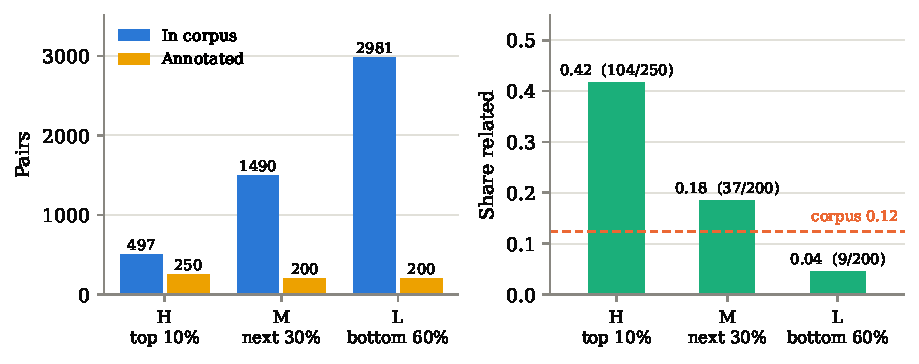
\includegraphics[width=\textwidth]{figures/stratum_yield}
\caption[Sampling strata and observed yield]{Left: size of each stratum in the
candidate space against the number of pairs annotated from it. Right: the share
of annotated pairs in each stratum carrying a relationship, with the
weighted corpus estimate for reference. The monotone gradient across strata is
evidence that the screening score orders the space as intended; the corpus
estimate sits below all but the lowest stratum because that stratum holds three
pairs in five.}
\label{fig:strata}
\end{figure}

Figure~\ref{fig:strata} shows the realised sample. The stratum yields (0.42,
0.18, 0.04) confirm the screening score separates the space, and they are also
why the design is efficient: an unstratified sample of the same size would spend
three annotations in five on a region where one pair in twenty-five is related.

One class stayed out of reach. The sample contains no \textsc{Equivalence} pair
at all, despite covering half of the top-decile stratum, so no weighted per-class
estimate can be given for it; the three instances in the corpus known to the
project all come from the purposive pilot. That is itself a measurement --- two
standards written for different layers of a system produce overlapping and
complementary obligations, but almost never identical ones --- and it is the
reason per-class results in Section~\ref{sec:classresults} are reported on the
pilot set only.

\subsection{Reliability of the reference set}\label{sec:gtvalidation}

Three statistics are reported, all computable from what was actually done. The
first is agreement between the sample and the author-reviewed pilot labels on the
pairs they share, using raw agreement and Cohen's kappa~\cite{cohen1960kappa}
with the bands of Landis and Koch~\cite{landis1977kappa}. The second is
calibration: whether recorded annotation confidence predicts where the two label
sets diverge. The third is a contrast rather than a validation --- the
run-to-run self-agreement of the evaluated LLM on identical input, which
establishes what an unreliable annotation source looks like on the same scale.

Cross-model agreement using Gemini is deliberately excluded. Gemini is one of the
evaluated methods, so its labels cannot serve as an independent check on a
reference set used to score it.

A larger validation with external cybersecurity professionals was designed but
not executed within the project timeframe; the complete survey instrument and
analysis plan are provided in Appendix~\ref{app:survey} as a ready-to-run
protocol for future work.

\section{Automated mapping methods}\label{sec:methods}

Eleven methods are evaluated, grouped into five families. The grouping is not
housekeeping: it is what the comparison is about. Lexical baselines match
words. Sentence-embedding models are trained so that cosine similarity means
something. Contextual-embedding models are masked language models pooled into a
vector without any such training. A cross-encoder reads both provisions at once
and answers a directional question. Hosted API models are the commercial
current generation. Differences within a family isolate the effect of the
model; differences between families isolate the effect of the approach.

\subsection{Rule-based baselines}

\paragraph{TF--IDF cosine similarity.} Each provision is represented as a
TF--IDF-weighted bag of words; every cross-standard pair receives the cosine
similarity of the two vectors. This captures shared vocabulary and nothing
else, making it the canonical lexical baseline.

\paragraph{Security-keyword Jaccard.} A curated list of cybersecurity terms
(password, authentication, encryption, vulnerability, logging, risk, update,
and others) is matched against each provision; a pair is scored by the Jaccard
overlap of the keyword sets. This baseline mimics how a checklist-driven
analyst might shortlist related provisions.

\subsection{Sentence-embedding models}

Three encoders trained so that cosine similarity between sentence embeddings
tracks semantic relatedness. Each provision is embedded once and every pair is
scored by the cosine of the two vectors.

\begin{itemize}
  \item \textbf{Sentence-BERT} (\texttt{all-MiniLM-L6-v2})
  ~\cite{reimers2019sbert}, the compact model that made this style of
  comparison cheap enough to run over a full pair space;
  \item \textbf{MPNet} (\texttt{all-mpnet-base-v2})~\cite{song2020mpnet}, the
  strongest general-purpose model of the same family, included so that the
  effect of model capacity can be separated from the effect of the task;
  \item \textbf{BGE} (\texttt{bge-base-en-v1.5})~\cite{xiao2024bge}, a
  retrieval-trained embedder a generation newer than the other two, included as
  the current state of the open embedding literature.
\end{itemize}

\subsection{Contextual-embedding models}

Three masked language models with no sentence-similarity training, mean-pooled
over token embeddings and L2-normalised. They are included to separate two
explanations for embedding performance that are easily confused --- the size of
the model, and whether it was ever trained to make its geometry mean something.

\begin{itemize}
  \item \textbf{BERT} (\texttt{bert-base-uncased})~\cite{devlin2019bert}, the
  general-purpose baseline;
  \item \textbf{SecureBERT}~\cite{aghaei2022securebert}, a
  cybersecurity-domain RoBERTa model;
  \item \textbf{CySecBERT}~\cite{bayer2024cysecbert}, a second, independently
  built cybersecurity-domain model. One domain-adapted model that behaves oddly
  is an anecdote about that model; two, adapted by different groups from
  different base models, make it a statement about domain adaptation for this
  task.
\end{itemize}

\subsection{Cross-encoder inference}\label{sec:nlimethod}

Every method above reduces a pair to one symmetric number, and a symmetric
number cannot say which of two provisions is the broader one. Subsumption is
therefore unreachable for all of them by construction. The
\textbf{NLI cross-encoder} (\texttt{nli-deberta-v3-base}, a DeBERTa-v3
model~\cite{he2023debertav3} fine-tuned on natural language inference
data~\cite{williams2018mnli}) reads both provisions together and returns
whether the first entails the second, which is a directional question.

Each pair is scored twice, once in each direction, and the two entailment
probabilities decide the label: entailment both ways is
\textsc{Equivalence}; entailment one way only is \textsc{Subsumption} with the
entailed provision as the narrower one; some entailment but not enough in
either direction is \textsc{Overlap}; and no entailment either way is
\textsc{No relation}. A direction counts as entailed at probability $0.50$, and
$0.20$ is the floor below which the method emits nothing at all. Both cut-offs
were fixed before any evaluation. The stored score is the larger of the two
entailment probabilities, so this method can be swept and recalibrated on the
same footing as the others. The cost is two forward passes per pair, 9{,}936 in
total, against one embedding pass per provision for the bi-encoders.

\subsection{Hosted API methods}

\paragraph{Gemini embeddings.} Each provision is embedded with Google's
\texttt{gemini-embedding-2} model via API; pairs are scored by cosine
similarity, exactly as for the local encoders. This represents the current
generation of commercial embedding models.

\paragraph{Gemini LLM classification.} For every one of the 4{,}968 pairs, a
prompt containing both provision texts and the six label definitions asks
\texttt{gemini-2.5-flash-lite} to answer with exactly one label. Jobs are
submitted through the batch API. Unlike the similarity methods, this approach
predicts a relationship type directly and can, in principle, distinguish
overlap from complementarity --- something a scalar similarity cannot.

\subsection{From similarity scores to labels}\label{sec:thresholds}

The similarity-based methods produce scores in $[0,1]$, not labels. Scores are
mapped to relationship types with fixed thresholds: $\geq 0.85$
\textsc{Equivalence}, $\geq 0.70$ \textsc{Overlap}, $\geq 0.50$
\textsc{Complementarity}, otherwise \textsc{No relation}. A second, lower
threshold decides whether a pair is emitted as a candidate at all, and it is
set per family rather than per model: $0.10$ and $0.05$ for the two lexical
baselines, $0.30$ for the sentence-embedding models, $0.70$ for the
contextual-embedding models, $0.50$ for the Gemini embeddings, and the
entailment floor of Section~\ref{sec:nlimethod} for the cross-encoder. These
cut-offs follow the operating points reported in related mapping work
~\cite{sapkota2016regcmantic}, and they are fixed per family rather than tuned
per model so that a difference between two models in the same family reflects
the representation and not the calibration.

That decision has a consequence worth stating in advance rather than
discovering in the results. A threshold chosen a priori is a threshold chosen
without knowing the base rate of related pairs, and
Section~\ref{sec:prevalence} shows the base rate is far lower than the pilot
set suggests. Several methods therefore ship at operating points that are badly
wrong for the corpus, which is why every method with a continuous score is also
reported at a threshold recalibrated on the probability sample. The threshold
sensitivity analysis in Section~\ref{sec:thresholdresults} shows how much of
each method's performance is representation and how much is calibration.

Subsumption cannot be expressed as a symmetric similarity band at all, so ten
of the eleven methods cannot predict it by construction. Only the cross-encoder
can, which is the reason it is in the study.

\section{Evaluation framework}\label{sec:evaluation}

Evaluation is restricted to the 107 annotated pairs; predictions outside the
annotated set are ignored, since their true labels are unknown. Two views are
computed for every method.

\subsection{Pair detection}

Detection asks whether a method finds related pairs at all, regardless of
label. A pair is a positive if its ground-truth label is anything but
\textsc{No relation}. With $TP$, $FP$, $FN$ counted within the annotated
scope:
\begin{equation}
  \text{Precision} = \frac{TP}{TP+FP}, \qquad
  \text{Recall} = \frac{TP}{TP+FN}, \qquad
  F_1 = \frac{2PR}{P+R}.
\end{equation}
One consequence of scoping deserves emphasis: false positives can only be
counted on the 22 annotated negative pairs. A method that predicts relations
sparsely can therefore show precision of 1.0 while missing nearly everything;
precision values must be read together with recall and with the
predicted-positive counts reported alongside.

\subsection{Relationship classification}

Classification asks whether the predicted label matches the ground truth,
over all 107 pairs, with the subsumption directions merged
(Section~\ref{sec:taxonomy}). Ground-truth pairs absent from a method's
output count as predicted \textsc{No relation}. Reported metrics are overall
accuracy and macro-averaged precision, recall, and F1 over the five classes,
plus per-class scores. Macro averaging weights all classes equally, which is
appropriate here because the rare classes (equivalence, subsumption) are
exactly the ones a compliance analyst cares most about.

\subsection{Uncertainty and sensitivity}

With 107 evaluation pairs, point estimates alone would overstate certainty.
Nonparametric bootstrap confidence intervals (2{,}000 resamples of the
annotated pairs, percentile method, 95\% level) are reported for detection F1
and macro-F1. For every method with a stored similarity matrix, detection
metrics are additionally computed across the full threshold range
$[0.05, 0.975]$ to separate the quality of the underlying representation from
the choice of operating point.

Corpus-level results are reported at two operating points, because the shipped
thresholds were selected on the pilot set and applying them to a corpus with a
different base rate confounds the method with its calibration. The second point
is chosen on the probability sample itself: weighted F1 is maximised on four
folds and scored on the fifth, over 20 repeats, with folds stratified by
sampling stratum so each carries all three weight classes. Candidate cut-offs
are quantiles of each method's own score distribution rather than a shared
absolute grid, since the methods occupy ranges that differ by an order of
magnitude in width. The reported threshold is the median of the 100 selections,
so the point estimate that follows is not the in-sample optimum; the gap between
it and the cross-validated mean is reported as the residual optimism.

Comparisons between methods use a paired bootstrap on the difference: both
methods are scored on the same within-stratum resample, and only differences
whose interval excludes zero are reported as orderings. Two marginal intervals
overlapping is not evidence that the methods are equivalent, because the
methods are scored on identical pairs and their errors are correlated.

Which comparisons are made is decided by a rule, not by inspection. Eleven
methods and their recalibrated variants admit more than two hundred pairwise
contrasts, and two hundred uncorrected 95\% intervals will contain false
findings whatever the data say. Two questions carry the argument --- whether a
method beats the all-positive baseline, and whether anything beats the
best-scoring method --- so each method is compared against those two references
and against nothing else. One caveat attaches to the second reference: it is
selected as the maximum on this sample, and a difference measured against a
selected maximum is biased in that maximum's favour, because the selection
absorbs part of the sampling noise. Those intervals describe the gap to the
leader; they are not a test that the leader is genuinely best.

\subsection{Efficiency and interpretability}

Wall-clock runtime of each stage is recorded on commodity hardware (Apple
silicon laptop, CPU only). Interpretability is assessed qualitatively: whether
a method's output carries any human-readable rationale (matched keywords, a
similarity score, or a generated label) that an analyst could act on.

\chapter{The Mapping Pipeline}\label{ch:prototype}

The methods of Chapter~\ref{ch:methodology} are implemented as a five-stage
pipeline, released as an open repository so that every number in
Chapter~\ref{ch:results} can be regenerated from the raw standard documents.
This chapter describes the system's structure, what was built for the project
and what was reused, and the artefacts each stage produces.

\section{Architecture}

\begin{figure}[htbp]
\centering
\begin{tikzpicture}[
  node distance=5mm and 7mm,
  stage/.style={draw, rounded corners=2pt, minimum height=9mm, minimum width=24mm,
                align=center, font=\small},
  art/.style={font=\scriptsize\itshape, align=center},
  arr/.style={-{Stealth[length=2.4mm]}, thick}
]
\node[stage] (ex) {Extraction};
\node[stage, right=of ex] (gt) {Ground\\truth};
\node[stage, right=of gt] (map) {Mapping\\(7 methods)};
\node[stage, right=of map] (ev) {Evaluation};
\node[stage, right=of ev] (rep) {Reporting};
\draw[arr] (ex) -- (gt);
\draw[arr] (gt) -- (map);
\draw[arr] (map) -- (ev);
\draw[arr] (ev) -- (rep);
\node[art, below=2.5mm of ex] {provision\\JSON};
\node[art, below=2.5mm of gt] {gt.csv\\(107 pairs)};
\node[art, below=2.5mm of map] {predictions,\\similarity matrices};
\node[art, below=2.5mm of ev] {metrics, errors,\\confidence intervals};
\node[art, below=2.5mm of rep] {tables,\\figures};
\end{tikzpicture}
\caption{Pipeline stages and the artefact each stage produces. Every stage is
a separate command, so intermediate outputs can be inspected before the next
stage runs.}
\label{fig:pipeline}
\end{figure}

Figure~\ref{fig:pipeline} shows the five stages. The pipeline is a set of
Python modules run stage by stage from the command line; each stage reads the
files of the previous one and writes its results to a versioned data
directory. This staged design was a deliberate choice over a single
end-to-end script: extraction errors are cheaper to catch before mapping runs,
and the API-based methods (which cost money per call) are only invoked once
their inputs are verified.

\section{Stage descriptions}

\paragraph{Extraction.} Converts both standard PDFs to text with
\texttt{pdftotext} (Poppler), removes recurring ETSI page furniture, locates
provision identifiers with pattern matching, and writes one JSON record per
provision with identifier, section, title, text, and modality. Output: 69
records for \standardA{}, 72 for \standardB{}.

\paragraph{Ground truth.} Materialises the reviewed annotation of
Section~\ref{sec:gt} as \texttt{gt.csv}: source and target provision
identifiers, one of six relationship labels, a one-sentence justification,
and a confidence score. A companion module draws the stratified probability
sample, emits and ingests the annotation batches, and computes the agreement
statistics of Section~\ref{sec:gtvalidation}.

\paragraph{Mapping.} One module per method. The rule-based module computes
TF--IDF cosine similarity (scikit-learn) and security-keyword Jaccard scores.
The three local transformer modules share a common embedding helper that
loads the model (Hugging Face), embeds all provisions, normalises the
vectors, and computes the full $69 \times 72$ cosine similarity matrix. The
Gemini embedding module obtains vectors through the Google GenAI API; the
Gemini classification module builds one prompt per pair and submits them
through the batch API, then parses the returned labels. Every
similarity-based module stores both its thresholded predictions (CSV) and its
raw similarity matrix (NumPy), the latter enabling the threshold sweep of
Section~\ref{sec:thresholdresults} without re-running any model.

\paragraph{Evaluation.} Loads the ground truth and every prediction file,
computes detection and classification metrics
(Section~\ref{sec:evaluation}), bootstrap confidence intervals, per-method
confusion matrices, and threshold sweeps, and writes per-method error files
listing every missed pair and every wrong label with its provision
identifiers.

\paragraph{Reporting.} Renders the summary tables and the figures used in
Chapter~\ref{ch:results} (matplotlib), in print-ready PDF form.

\section{Built versus reused}

The extraction logic, the keyword baseline, the ground-truth tooling, the
evaluation harness with its bootstrap and sweep analyses, and the reporting
layer were developed for this project. The heavy lifting inside the mapping
methods deliberately reuses standard components: scikit-learn's TF--IDF
vectoriser, pretrained models from Hugging Face (MiniLM Sentence-BERT, BERT
base, SecureBERT), and Google's hosted Gemini models. No model was trained or
fine-tuned; assembling and evaluating existing components under controlled,
identical conditions is precisely the contribution.

\section{Reproducibility}

All randomised steps (sampling, bootstrap) use fixed seeds. A verification run
during the project reproduced every stored evaluation metric exactly;
individual embedding scores vary in the fourth decimal between runs because of
CPU thread scheduling in the tensor library, which never crosses a label
threshold. The API-based methods depend on hosted models and are archived
through their stored outputs instead. Appendix~\ref{app:reproduction} lists the exact commands, software
versions, and expected runtimes for a full reproduction.

\chapter{Results and Discussion}\label{ch:results}

This chapter reports the experimental results. Section~\ref{sec:setup} recalls
the setup, Sections~\ref{sec:detectionresults}--\ref{sec:classresults} present
pair detection, similarity structure, threshold sensitivity, and relationship
classification, Section~\ref{sec:agreementresults} covers the ground-truth
validation study, and Sections~\ref{sec:efficiency}--\ref{sec:threats} discuss
the findings against the research questions and the threats to their validity.

\section{Experimental setup}\label{sec:setup}

All eleven methods were run on the full cross product of 69 \standardA{}
provisions and 72 \standardB{} provisions (4{,}968 pairs) and evaluated on
the 107 annotated pairs: 85 related pairs and 22 annotated negatives
(Figure~\ref{fig:gtdist}). The distribution is dominated by \textsc{Overlap}
(51 pairs), with \textsc{Equivalence} rare (3 pairs) --- the two standards
describe different system layers, so identical requirements barely occur.
Metrics outside the annotated scope are not computable and are not claimed.

\begin{figure}[htbp]
\centering
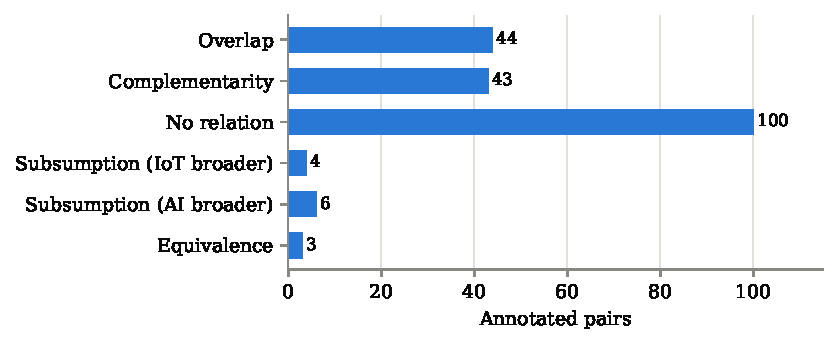
\includegraphics[width=0.72\textwidth]{figures/gt_distribution}
\caption{Distribution of relationship labels in the 107-pair ground truth.}
\label{fig:gtdist}
\end{figure}

\section{Pair detection}\label{sec:detectionresults}

Table~\ref{tab:detection} and Figure~\ref{fig:detectionbars} show the
detection results; Figure~\ref{fig:cis} adds bootstrap confidence intervals.

\begin{table}[htbp]
\centering
\caption{Pair detection on the annotated scope. $P^{+}$ is the number of
pairs the method marks as related among the 107 annotated pairs. Precision
counts false positives only on the 22 annotated negatives, which is why
sparse methods show precision 1.00 despite very low recall.}
\label{tab:detection}
\small
\begin{tabular}{lrrrrrrr}
\toprule
Method & $P^{+}$ & TP & FP & FN & Precision & Recall & F1\\
\midrule
TF--IDF            &   3 &  3 &  0 & 82 & 1.000 & 0.035 & 0.068\\
Keyword Jaccard    &   6 &  6 &  0 & 79 & 1.000 & 0.071 & 0.132\\
Sentence-BERT      &  15 & 15 &  0 & 70 & 1.000 & 0.176 & 0.300\\
MPNet              &  14 & 14 &  0 & 71 & 1.000 & 0.165 & 0.283\\
BGE                &  90 & 75 & 15 & 10 & 0.833 & 0.882 & 0.857\\
BERT               & 105 & 85 & 20 &  0 & 0.809 & 1.000 & \textbf{0.895}\\
SecureBERT         & 107 & 85 & 22 &  0 & 0.794 & 1.000 & 0.885\\
CySecBERT          & 107 & 85 & 22 &  0 & 0.794 & 1.000 & 0.885\\
NLI cross-encoder  &   5 &  5 &  0 & 80 & 1.000 & 0.059 & 0.111\\
Gemini embeddings  & 107 & 85 & 22 &  0 & 0.794 & 1.000 & 0.885\\
Gemini LLM         &  94 & 73 & 21 & 12 & 0.777 & 0.859 & 0.816\\
\bottomrule
\end{tabular}
\end{table}

\begin{figure}[htbp]
\centering
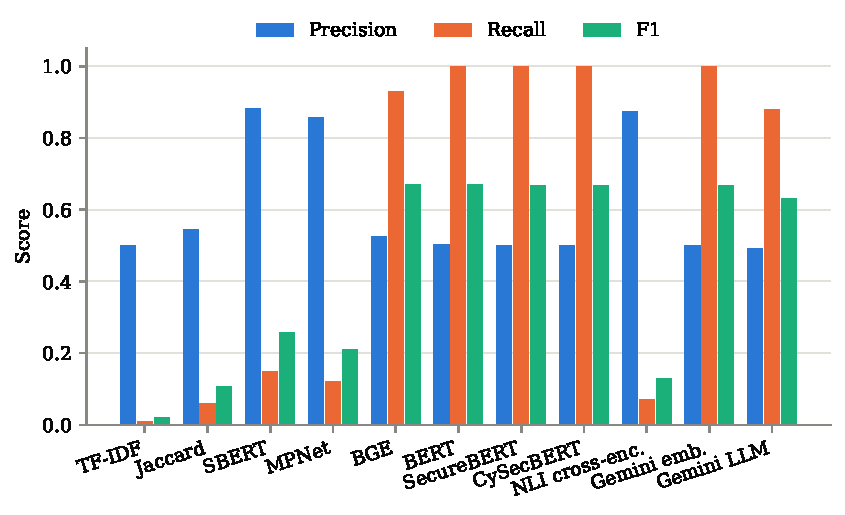
\includegraphics[width=0.9\textwidth]{figures/detection_metrics}
\caption{Pair-detection precision, recall, and F1 per method.}
\label{fig:detectionbars}
\end{figure}

\begin{figure}[htbp]
\centering
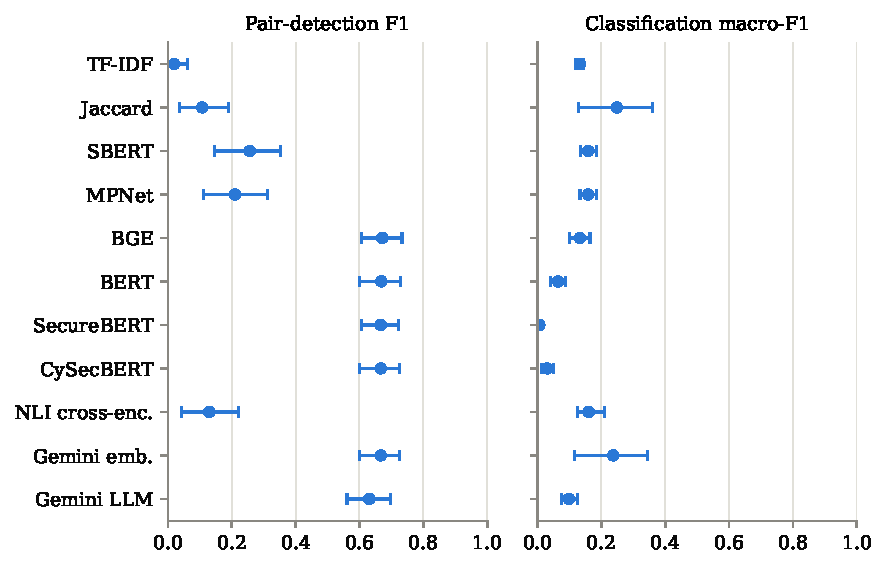
\includegraphics[width=\textwidth]{figures/f1_confidence_intervals}
\caption{Bootstrap 95\% confidence intervals (2{,}000 resamples) for
pair-detection F1 and classification macro-F1.}
\label{fig:cis}
\end{figure}

The table splits the methods into two regimes. The lexical baselines and
Sentence-BERT at its default operating point predict very few relations; what
they do predict is correct (no false positives), but recall between 0.02 and
0.17 makes them useless as stand-alone detectors. The remaining methods sit at
the opposite extreme. SecureBERT and Gemini embeddings mark \emph{every}
annotated pair as related, and BERT marks all but two. Their high F1
($\approx$0.89) must therefore be read with care: with 85 of 107 annotated
pairs being positives, the trivial strategy ``call everything related''
already achieves F1 = 0.885. BERT, SecureBERT, and Gemini embeddings
essentially implement that strategy, and the Gemini LLM (F1 = 0.816) stays
below it. Detection F1 within the annotated scope, in other words, barely
distinguishes these methods; the informative differences appear in the
similarity structure and in classification.

\section{Similarity structure}\label{sec:simstructure}

\begin{figure}[htbp]
\centering
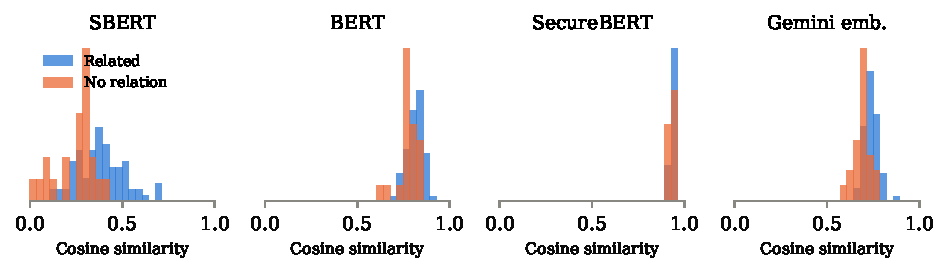
\includegraphics[width=\textwidth]{figures/similarity_distributions}
\caption{Score distributions for annotated related pairs (blue) and annotated
negatives (orange), one panel per method with a continuous score. Panels are
not on a common scale: what matters is the separation between the two
distributions within a panel, not where either sits.}
\label{fig:simdist}
\end{figure}

Figure~\ref{fig:simdist} explains the degenerate behaviour, and with eleven
methods the pattern is legible as a family property rather than a quirk of one
model. All three contextual-embedding models compress: BERT places every pair,
related or not, between roughly 0.57 and 0.91; CySecBERT between 0.71 and 0.93;
SecureBERT is the extreme case, packing the entire corpus into
$[0.875, 0.971]$, a band 0.10 wide. With ranges that narrow, the fixed label
thresholds of Section~\ref{sec:thresholds} land every pair in the same band:
SecureBERT assigns \textsc{Equivalence} to all 4{,}968 possible pairs, and
CySecBERT splits them between \textsc{Equivalence} and \textsc{Overlap} without
ever reaching \textsc{No relation}. This matches the known anisotropy of
contextual embedding spaces~\cite{ethayarajh2019contextual}: mean-pooled vectors
from models never trained for sentence similarity crowd into a narrow cone, and
cosine similarity loses its discriminative meaning. Adding cybersecurity
vocabulary does not repair the geometry --- both domain-adapted models are more
compressed than the general-purpose model they descend from, not less.

The sentence-embedding models spread out, as their training intends.
Sentence-BERT and MPNet span roughly $[-0.05, 0.8]$ and visibly separate the two
distributions --- yet even there the overlap is substantial, confirming that
annotated negatives (chosen to share surface vocabulary) are genuinely hard.
BGE is the instructive intermediate: it is trained for similarity and separates
the classes well, but its scores never fall below 0.345, so a threshold chosen
for its family lands beneath its entire distribution. Its saturation is an
artefact of where its scores sit, not of what they encode --- which is exactly
the distinction the recalibration in Section~\ref{sec:prevalence} isolates.
Gemini embeddings sit between the extremes: compressed range, but with related
pairs shifted consistently above negatives. The NLI cross-encoder is unlike all
of them, producing a probability rather than a cosine and placing the bulk of
pairs near zero, which is why its panel looks empty on the right.

\section{Threshold sensitivity}\label{sec:thresholdresults}

\begin{figure}[htbp]
\centering
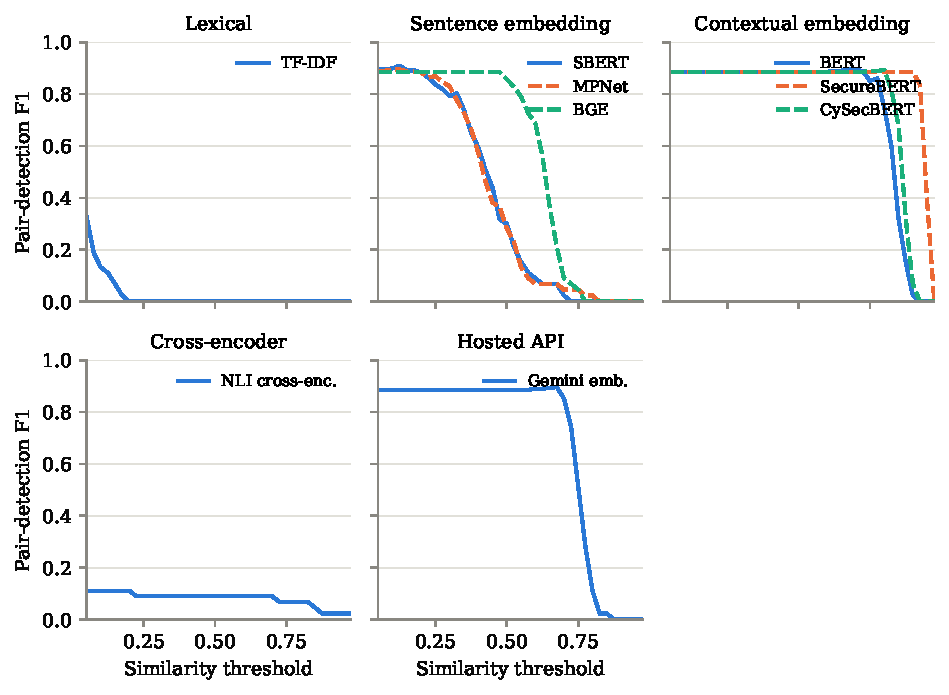
\includegraphics[width=0.78\textwidth]{figures/threshold_sweep}
\caption{Pair-detection F1 as a function of the decision threshold, computed
from the stored score matrices on the annotated scope, faceted by method
family. Eleven curves on shared axes cannot be distinguished by colour, and the
families are what the comparison is about.}
\label{fig:sweep}
\end{figure}

Figure~\ref{fig:sweep} separates representation quality from the choice of
operating point. Three observations stand out. First, the plateaus of BERT,
SecureBERT, and Gemini embeddings coincide with the all-positive baseline
(F1 $\approx$ 0.885) across most of the threshold range --- confirming that
their default-threshold results reflect saturation, not discrimination.
CySecBERT joins them, and the faceting makes the point sharper than a single
axis would: every member of the contextual-embedding panel shows the same
plateau, while no member of the sentence-embedding panel does.
Second, with an optimally chosen threshold Sentence-BERT becomes the
\emph{best} detector (F1 = 0.909 at $t=0.120$), despite being the worst
non-trivial one at its default operating point; MPNet and BGE reach 0.895 and
0.897 on the same basis, so the three sentence-embedding models are effectively
tied once their operating points are chosen properly. Their published default
entry thresholds are simply the wrong ones for cross-standard requirement
text. Choosing a
threshold on the same pairs the score is reported on inflates it, so the sweep
was repeated under 5-fold cross-validation with 20 repetitions: the threshold is
selected on four folds and scored on the fifth. Held-out F1 is
$0.903 \pm 0.021$, an optimism of only 0.006, because a single tuned parameter
over 107 points has little room to overfit.
Figure~\ref{fig:cvthreshold} shows the same comparison for every method with a
continuous score, together with the spread of the selected threshold itself. The
two panels carry different news: held-out F1 tracks the in-sample optimum closely
everywhere, but the threshold that produces it is stable only for some models.
Gemini embeddings settle on $0.658 \pm 0.023$ across all 100 fits, whereas
SecureBERT ranges over $0.265 \pm 0.375$ --- its folds disagree about the
operating point by more than the width of the useful range, which is the same
brittleness the sweep curve shows from a different angle.
Calibration gain is therefore real,
though Section~\ref{sec:prevalence} shows it is measured at a positive rate the
corpus does not share. Third,
the sharp cliffs on the right show how brittle threshold-based labelling is:
for SecureBERT the entire working range collapses within a few hundredths.
For practice this means thresholds must be calibrated per corpus and per
model --- fixed literature values do not transfer.

\begin{figure}[htbp]
\centering
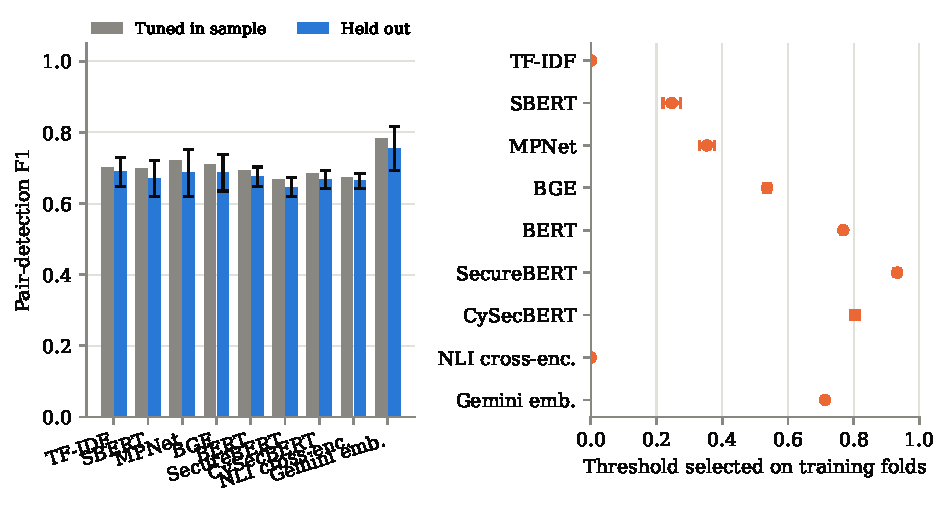
\includegraphics[width=\textwidth]{figures/cv_threshold}
\caption[Cross-validated threshold calibration]{Left: pair-detection F1 with the
threshold tuned on the same pairs it is scored on, against the held-out mean of
20 repeats of stratified 5-fold cross-validation (error bars, one standard
deviation). Right: the threshold each set of training folds selected.}
\label{fig:cvthreshold}
\end{figure}

\section{Corpus-level performance}\label{sec:prevalence}

Every figure reported so far describes the 107 pilot pairs, of which 85 are
related --- a positive rate of 79.4\%. That set was assembled purposively, so it
carries no inclusion probabilities and its precision cannot be reweighted to the
corpus it was drawn from. Because precision and F1 both move with the positive
rate, this matters: a method evaluated where four pairs in five are related is
being asked an easier question than the one it would face in use.

To measure rather than assume the difference, a stratified probability sample of
the full $69\times72$ space was drawn and annotated independently
(Section~\ref{sec:sampling}). Each pair carries a known inclusion probability, so
Horvitz--Thompson estimation recovers corpus-level quantities with correct
variance.

\paragraph{How common are related pairs?} The sample puts the corpus rate at
\textbf{12.4\%} (95\% CI [10.0, 15.0]) for any relationship, and \textbf{5.9\%}
(95\% CI [4.3, 7.7]) counting only equivalence, overlap and subsumption. Applied
to 4{,}968 candidates that implies roughly 617 and 295 related pairs
respectively. The pilot's 85 was never a measurement of this quantity --- it was
the number of pairs that study examined.

The unequal sampling fractions cost some precision of their own. With weights
ranging from 1.99 to 14.91, Kish's design effect is 1.49, so the 650 annotated
pairs carry the information of roughly 437 drawn with equal probability. Every
interval reported below already accounts for this, because the bootstrap
resamples within stratum.

\begin{table}[htbp]
\centering
\caption[Corpus-level detection performance]{Detection performance estimated over
all 4{,}968 candidate pairs from the weighted sample, at each method's shipped
operating point. Specificity is the fraction of unrelated pairs correctly
rejected. The final row is a classifier that labels every pair related.}
\label{tab:weighted}
\small
\begin{tabular}{lcccc}
\toprule
Method & Precision & Recall & Specificity & F1\\
\midrule
TF--IDF                 & 0.000 & 0.000 & 1.000 & 0.000\\
Keyword Jaccard         & 0.101 & 0.019 & 0.976 & 0.033\\
Sentence-BERT           & \textbf{0.905} & 0.061 & 0.999 & 0.115\\
MPNet                   & 0.696 & 0.057 & 0.997 & 0.106\\
BGE                     & 0.147 & 0.867 & 0.289 & \textbf{0.252}\\
BERT                    & 0.128 & 1.000 & 0.038 & 0.228\\
SecureBERT              & 0.124 & 1.000 & 0.000 & 0.221\\
CySecBERT               & 0.124 & 1.000 & 0.000 & 0.221\\
NLI cross-encoder       & 0.129 & 0.027 & 0.974 & 0.045\\
Gemini embeddings       & 0.124 & 1.000 & 0.000 & 0.221\\
Gemini LLM              & 0.121 & 0.886 & 0.092 & 0.214\\
\midrule
\emph{Label every pair related} & \emph{0.124} & \emph{1.000} & \emph{0.000} & \emph{0.221}\\
\bottomrule
\end{tabular}
\end{table}

\paragraph{The ranking inverts.} Table~\ref{tab:weighted} does not rearrange the
pilot ordering so much as contradict it. SecureBERT, CySecBERT and Gemini
embeddings reach specificity 0.000: across the weighted sample they reject no
unrelated pair at all, and their scores match the all-positive baseline to three
decimals. BERT, which led the pilot benchmark at detection F1 0.895, rejects
3.8\% of unrelated pairs. A paired bootstrap on the difference in F1 --- both
methods scored on the same resampled pairs, which is the comparison the overlap
of two marginal intervals does not make --- leaves four of the eleven methods
inside the baseline's interval: SecureBERT, CySecBERT and Gemini embeddings at
exactly zero difference, and the Gemini LLM at $-0.007$ [$-0.025$, 0.009]. BERT
sits ahead of the baseline by 0.007 [0.003, 0.011], a margin with no practical
content.

Sentence-BERT and MPNet move the other way. Both looked mediocre on the pilot set
(F1 0.300 and 0.283) and are the only methods here with precision of practical
interest: 0.905 and 0.696, meaning most of what they surface is genuinely
related. They pay for it with recall near 0.06. The NLI cross-encoder behaves
the same way from the other end of the design space --- precision 0.129 at recall
0.027 --- and BGE, alone among the sentence-embedding models, lands in the
saturated regime instead, flagging 87\% of the corpus.

That split runs along family lines, and it is the clearest structural finding
of the corpus view. The three models never trained for sentence similarity
(BERT, SecureBERT, CySecBERT) all saturate. Two of the three trained for it
(Sentence-BERT, MPNet) do the opposite and become too conservative to be useful.
Neither behaviour is about the model's size or its domain; both are about
whether its score distribution happens to straddle the threshold it inherited.

Sensitivity and specificity are properties of a classifier alone; precision also
depends on how common the positive class is. Fixing the first two therefore fixes
precision as a function of prevalence, plotted in
Figure~\ref{fig:precprev}. Three of the four methods shown lie on the diagonal
$\text{precision} = \text{prevalence}$, the locus of a classifier that carries no
information about the label: at the pilot's 0.79 they return 0.79, which reads as
strong performance, and at the corpus rate of 0.12 they return 0.12. Only
Sentence-BERT's curve stands away from the diagonal, and it is the separation
between curve and diagonal --- not the height of either --- that measures
discrimination.

\begin{figure}[htbp]
\centering
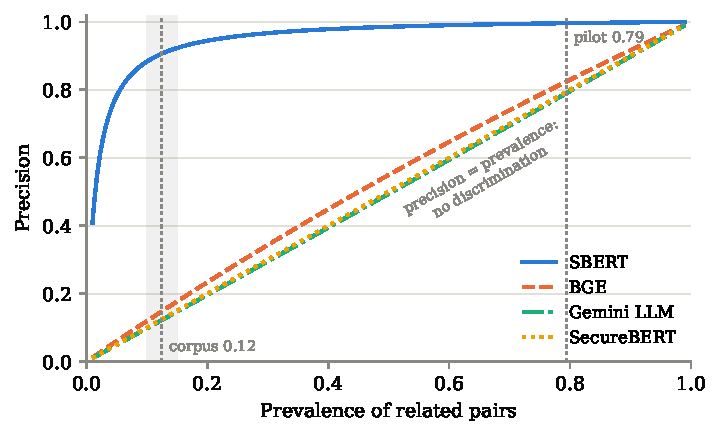
\includegraphics[width=0.78\textwidth]{figures/precision_vs_prevalence}
\caption[Precision as a function of prevalence]{Precision implied by each
method's estimated sensitivity and specificity as the share of related pairs
varies. Dotted lines mark the pilot set's positive rate and the corpus estimate;
the shaded band is the 95\% interval on the latter.}
\label{fig:precprev}
\end{figure}

\paragraph{How much of the collapse is the threshold?} Table~\ref{tab:weighted}
scores each method at the operating point Chapter~\ref{ch:prototype} shipped, and
those thresholds were chosen on the pilot set. Selecting a cut-off where 79\% of
pairs are related and then applying it where 12\% are confounds the method with
its calibration, so the comparison was repeated with the operating point selected
on the probability sample itself: weighted F1 maximised on four folds and scored
on the fifth, 20 repeats, stratified so every fold carries all three strata, with
the reported threshold the median of the 100 selections rather than the in-sample
optimum. Candidate cut-offs are quantiles of each method's own scores, since the
methods occupy very different ranges --- TF--IDF tops out at 0.14 while SecureBERT
never drops below 0.91, and a shared absolute grid would give one of them a
hundred candidate thresholds and the other three.

\begin{table}[htbp]
\centering
\caption[Corpus performance at a corpus-calibrated operating point]{Detection
performance when the threshold is selected on the probability sample instead of
the pilot set. Held-out F1 is the cross-validated mean; the gap to the point
estimate is the remaining optimism.}
\label{tab:calibrated}
\small
\begin{tabular}{lccccc}
\toprule
Method & Threshold & Precision & Recall & F1 & Held-out F1\\
\midrule
Gemini embeddings & 0.719 & \textbf{0.446} & 0.571 & \textbf{0.501} & 0.485\\
BGE               & 0.578 & 0.360 & 0.570 & 0.441 & 0.413\\
MPNet             & 0.325 & 0.336 & 0.611 & 0.434 & 0.405\\
Sentence-BERT     & 0.324 & 0.327 & 0.571 & 0.416 & 0.378\\
TF--IDF           & 0.017 & 0.281 & 0.367 & 0.319 & 0.285\\
BERT              & 0.824 & 0.233 & 0.477 & 0.313 & 0.289\\
CySecBERT         & 0.857 & 0.204 & 0.497 & 0.289 & 0.274\\
SecureBERT        & 0.939 & 0.178 & 0.508 & 0.264 & 0.252\\
NLI cross-encoder & 0.002 & 0.194 & 0.334 & 0.246 & 0.211\\
\midrule
\emph{Label every pair related} & --- & \emph{0.124} & \emph{1.000} & \emph{0.221} & ---\\
\bottomrule
\end{tabular}
\end{table}

The result changes the diagnosis (Figure~\ref{fig:calibgap}). At a threshold
fitted to the corpus, seven of the nine continuous methods clear the all-positive
baseline by a margin the paired bootstrap separates from zero. Gemini embeddings
lead at $+0.280$ [0.204, 0.362], with BGE at $+0.221$ [0.145, 0.295], MPNet at
$+0.213$ [0.146, 0.282] and Sentence-BERT at $+0.195$ [0.126, 0.267] behind it.
TF--IDF, BERT and CySecBERT beat it by 0.098, 0.093 and 0.068, intervals
excluding zero but only just. Two do not clear it at all: SecureBERT
($+0.043$, [$-0.009$, 0.095]) and the NLI cross-encoder
($+0.025$, [$-0.049$, 0.098]).

The top of that ranking is a four-way tie rather than a winner. Measured against
the leader, BGE ($-0.060$, [$-0.161$, 0.045]), MPNet ($-0.067$, [$-0.160$,
0.019]) and Sentence-BERT ($-0.085$, [$-0.184$, 0.015]) all have intervals
containing zero, so the honest statement is that a hosted commercial embedding
and three freely available local models cannot be told apart on this task. That
matters practically: the best local model matches the paid one within the
resolution this sample supports.

What collapsed in Table~\ref{tab:weighted}, then, was mostly calibration rather
than representation. The embedding spaces do carry enough signal to reject
unrelated pairs; the thresholds inherited from a 79\%-positive development set
did not let them. That is a sharper version of the same warning: the cost of a
development set at the wrong base rate is not a mild optimism in the reported
score, it is an operating point that turns a usable model into a constant
function. SecureBERT is the exception, and the informative one --- its scores
occupy a band 0.06 wide across the entire corpus, so no threshold placed anywhere
in that band separates the classes. CySecBERT, adapted to the same domain from a
different base model by a different group, is the near-exception: it recovers
enough range to clear the baseline by 0.068, but still finishes below plain BERT.
Two independent attempts at cybersecurity domain adaptation both end up worse
than the general-purpose model they were built from, which is a stronger
statement than either could make alone.

\begin{figure}[htbp]
\centering
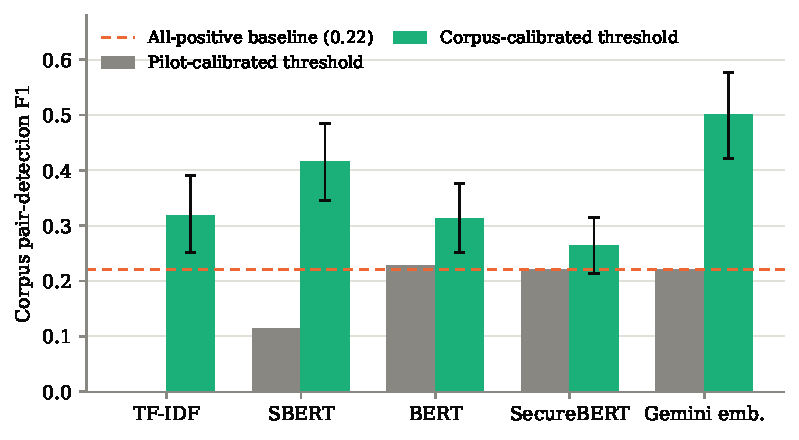
\includegraphics[width=0.82\textwidth]{figures/calibration_gap}
\caption[Effect of recalibrating the operating point]{Corpus pair-detection F1 at
the shipped, pilot-calibrated threshold against a threshold cross-validated on
the probability sample. Error bars are stratified bootstrap 95\% intervals.}
\label{fig:calibgap}
\end{figure}

\paragraph{What this supports.} Even recalibrated, no method here supports an
automated accept/reject decision: the best F1 is 0.50, with precision 0.45, so
more than half of what the system proposes is wrong. The defensible use is the
one Section~\ref{sec:discussion} describes --- ranking candidates for a human
reviewer --- and the choice of configuration depends on which end of the trade-off
matters. Sentence-BERT at its shipped threshold surfaces few pairs but is right
about nine times in ten; Gemini embeddings recalibrated recover 57\% of the
related pairs at under half precision. Neither removes the reviewer.

\section{Relationship classification}\label{sec:classresults}

Detecting that two provisions relate is only half the task; compliance work
needs to know \emph{how} they relate. Table~\ref{tab:classification}
summarises classification performance.

\begin{table}[htbp]
\centering
\caption{Relationship classification over all 107 annotated pairs, five-label
scheme (subsumption directions merged). CIs are bootstrap 95\% intervals.}
\label{tab:classification}
\small
\begin{tabular}{lccc}
\toprule
Method & Accuracy & Macro-F1 & Macro-F1 95\% CI\\
\midrule
TF--IDF            & 0.215 & 0.086 & [0.053, 0.128]\\
Keyword Jaccard    & 0.224 & 0.179 & [0.059, 0.288]\\
Sentence-BERT      & 0.224 & 0.099 & [0.064, 0.137]\\
MPNet              & 0.224 & 0.100 & [0.064, 0.140]\\
BGE                & 0.243 & 0.149 & [0.098, 0.199]\\
BERT               & 0.411 & 0.172 & [0.114, 0.234]\\
SecureBERT         & 0.028 & 0.011 & [0.000, 0.025]\\
CySecBERT          & 0.196 & 0.087 & [0.057, 0.118]\\
NLI cross-encoder  & 0.215 & 0.102 & [0.054, 0.164]\\
Gemini embeddings  & \textbf{0.477} & \textbf{0.279} & [0.150, 0.388]\\
Gemini LLM         & 0.187 & 0.088 & [0.052, 0.127]\\
\bottomrule
\end{tabular}
\end{table}

\begin{figure}[htbp]
\centering
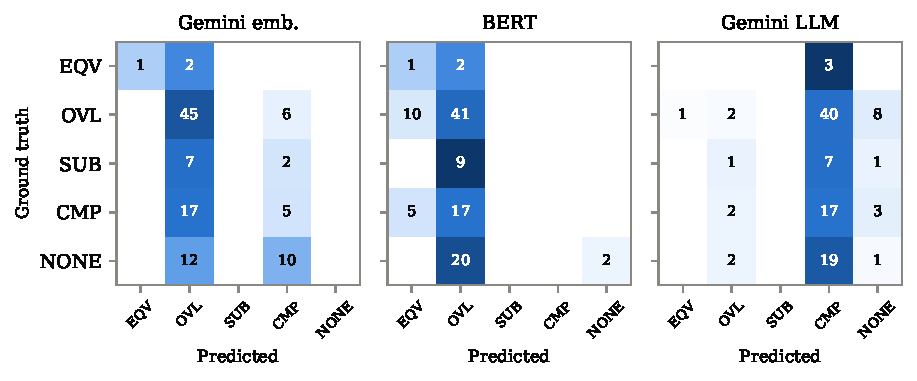
\includegraphics[width=\textwidth]{figures/confusion_matrices}
\caption{Row-normalised confusion matrices (counts printed) for the most
instructive methods, one per family. EQV = equivalence, OVL = overlap, SUB = subsumption,
CMP = complementarity, NONE = no relation.}
\label{fig:confusion}
\end{figure}

Classification is where every method struggles. The best result --- Gemini
embeddings at 0.477 accuracy and 0.279 macro-F1 --- would still mislabel every
second pair. The comparison that matters is against the trivial classifier
that assigns the majority label to everything: \textsc{Overlap} accounts for
51 of the 107 pairs, so always predicting it yields 0.477 accuracy. The best
method matches that figure exactly and none exceeds it. The same baseline
scores 0.129 macro-F1, which four methods do beat --- keyword Jaccard, BGE, BERT
and Gemini embeddings --- so the methods are not uniformly worthless; but the
headline conclusion has to be stated plainly. On the five-label task, none of the eleven methods learns the
distinction the task is about. The confusion matrices in
Figure~\ref{fig:confusion} show how each one fails:

\begin{itemize}
  \item \textbf{Gemini embeddings} funnel most predictions into
  \textsc{Overlap}. That matches the majority class (hence the comparatively
  high accuracy) and yields reasonable per-class scores for \textsc{Overlap}
  (F1 = 0.65) and \textsc{Equivalence} (precision 1.00 at recall 0.33), but
  \textsc{Subsumption} and \textsc{No relation} are never predicted
  correctly.
  \item \textbf{BERT} spreads slightly more but shows the same collapse;
  \textsc{Complementarity} and \textsc{Subsumption} both go to zero.
  \item \textbf{The Gemini LLM} is the only method that predicts labels from
  provision content rather than a score band, and it does recognise
  complementarity (recall 0.59) --- but it heavily overuses it, pushing 41 of
  the 51 \textsc{Overlap} pairs into \textsc{Complementarity} and ending with
  the lowest accuracy of the non-degenerate methods. Notably, it also assigns
  a relation to 20 of the 22 annotated negatives.
  \item \textbf{SecureBERT}'s uniform \textsc{Equivalence} output produces
  0.028 accuracy --- exactly the 3 equivalence pairs in the ground truth.
  \item \textbf{The NLI cross-encoder} is the only method that predicts
  \textsc{Subsumption} at all. Over the full corpus it emits 123 subsumption
  labels where every other method emits none, because every other method scores
  pairs with a symmetric function and direction is not recoverable from one. Its
  macro-F1 of 0.102 is nonetheless unremarkable, and the reason is instructive:
  it is extremely conservative, flagging 142 of 4{,}968 pairs, so it reaches the
  directional label on too few pairs to score well. The capability is real and
  the recall is not. This is the one structural gap in the taxonomy that a
  different architecture --- rather than a better-calibrated threshold --- does
  close, which is why it is worth reporting despite the weak headline number.
\end{itemize}

Two error examples illustrate the pattern. Provision 5.3-11 of \standardA{}
(inform the user that a security update is required, with its risks) and
provision 5.3.1-2.2 of \standardB{} (proactively inform end-users of
security-relevant updates with clear explanations) are annotated
\textsc{Equivalence}; Gemini embeddings scored the pair into the
\textsc{Overlap} band --- a near-miss that a human reviewer would accept as a
shortlist hit. By contrast, the Gemini LLM labelled the pair of provision
5.1-1 (unique per-device passwords) and provision 5.2.2-1 (evaluate access
control frameworks for APIs, models, and data) as \textsc{Complementarity}
where the annotation says \textsc{Overlap}: both provisions govern
authentication-related access control, but the model read the difference in
system layer as a difference in objective. The boundary between overlap and
complementarity is exactly where the annotation itself is hardest, a point
the validation study below quantifies.

\section{Coverage and gaps}\label{sec:coverage}

The preceding sections measure how often a method is right. This one asks what
the method actually says about the two standards, which is the question a
compliance practitioner brings to a mapping exercise: which provisions of
\standardA{} have a counterpart in \standardB{}, and which have none. The
manual study closest to this one~\cite{djebbar2023comparative} reports exactly
that --- a coverage statement and an explicit list of unmapped requirements ---
so producing the same two artefacts automatically is the fairest way to show
what the automation delivers.

Everything in this section is a prediction from a single method, the
best-scoring one at its corpus-calibrated operating point, and its precision at
that point is 0.446 with a 95\% interval of [0.362, 0.535]. Roughly half of
what follows is therefore wrong. The section is included because a shortlist
with a known error rate is a usable artefact and a mapping with an unknown one
is not, but nothing here carries the standing of the estimates in
Section~\ref{sec:prevalence}.

At its calibrated threshold the method flags 797 of the 4{,}968 candidate pairs,
16.0\% of the space, against an estimated true prevalence of 12.4\%
[10.0\%, 15.0\%]. It over-predicts, which is what a threshold chosen to maximise
F1 at a low base rate should do: recall is worth more than precision when the
output is a shortlist for human review.

\begin{figure}[htbp]
  \centering
  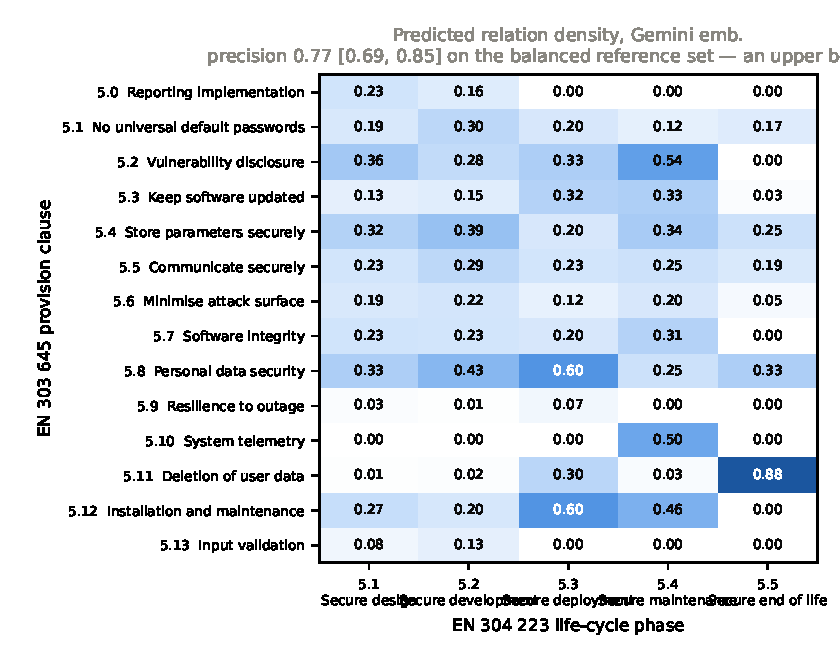
\includegraphics[width=0.82\linewidth]{figures/coverage_heatmap.pdf}
  \caption{Predicted relation density by clause. Each cell is the share of
  provision pairs in that clause block flagged as related by Gemini embeddings
  at the corpus-calibrated threshold of 0.719. These are predictions, not
  verified relations: the method's precision at this operating point is 0.446
  [0.362, 0.535].}
  \label{fig:coverage}
\end{figure}

Figure~\ref{fig:coverage} shows where the predicted relations concentrate. The
density is uneven in a way that follows the structure of the two documents
rather than the behaviour of the model.

The gap side is the more informative one, and it is the part a similarity
threshold can state cleanly. Eight of the 69 \standardA{} provisions and five
of the 72 \standardB{} provisions receive no predicted counterpart at all;
Table~\ref{tab:unmapped} lists them. A gap here is a weaker claim than a gap in
a manual study: it means the method found nothing, not that nothing is there,
and at a recall well below one the two are different statements. The list is
useful in the direction that a false gap is cheap to check --- an analyst reads
thirteen provisions --- and expensive to miss.

\begin{table}[htbp]
  \centering
  \caption{Provisions with no predicted counterpart in the other standard, at
  the corpus-calibrated operating point. Absence of a prediction is not evidence
  of absence of a relation; the method's recall at this threshold is below one.}
  \label{tab:unmapped}
  \small
  % Generated by src.evaluation.coverage -- do not edit by hand.
\begin{tabular}{@{}llp{0.60\linewidth}@{}}
\toprule
Standard & Provision & Requirement \\
\midrule
EN 303 645 & 5.1-2A & Passwords should not be used for machine-to-machine authentication. Using human-memorable p\textbackslash{}ldots \\
 & 5.3-15A & For devices that cannot have their software updated, the consumer IoT device should be isol\textbackslash{}ldots \\
 & 5.5-3 & Cryptographic algorithms and primitives should be replaceable. \\
 & 5.5-4 & Access to consumer IoT device functionality via a network interface in the initialized stat\textbackslash{}ldots \\
 & 5.6-4B & Debug interfaces that are physical ports should be physically protected by the device. \\
 & 5.6-6 & Code should be minimized to the functionality necessary for the consumer IoT device to oper\textbackslash{}ldots \\
 & 5.9-2 & Consumer IoT devices should remain operating and locally functional in the case of a loss o\textbackslash{}ldots \\
 & 5.9-3 & The consumer IoT device should connect to networks in an expected, operational and stable s\textbackslash{}ldots \\
\midrule
EN 304 223 & 5.1.1-1.1 & AI security training shall be tailored to the specific roles and responsibilities of staff\textbackslash{}ldots \\
 & 5.1.2-1.1 & Where the Data Custodian is part of a Developer's organization, they shall be included in i\textbackslash{}ldots \\
 & 5.1.3-1.3 & System Operators shall apply controls to risks identified through the analysis based on a r\textbackslash{}ldots \\
 & 5.2.3-3 & Developers and System Operators shall re-run evaluations on released models that they inten\textbackslash{}ldots \\
 & 5.2.5-2 & System Operators shall conduct testing prior to the system being deployed with support from\textbackslash{}ldots \\
\bottomrule
\end{tabular}

\end{table}

The full predicted mapping --- all 797 pairs with their scores --- is given in
Appendix~\ref{app:mapping}. Both the table above and that appendix are
generated directly from the evaluation outputs, so neither can drift from the
numbers reported here.

\section{Ground-truth validation}\label{sec:agreementresults}

A reference set is only as good as the consistency of the judgements behind it.
The pilot pairs were mixed unmarked into the annotation stream for the
probability sample, so re-labelling them was blind: at the time of judging, there
was no way to tell a pilot pair from a newly sampled one. Comparing the two label
sets afterwards gives an agreement figure against annotations that two authors
reviewed months earlier.

\begin{table}[htbp]
\centering
\caption[Reference-set agreement against the pilot and the LLM contrast]{%
Agreement of the annotated reference sample with the earlier author-reviewed
pilot labels, against the same statistic computed for the evaluated LLM on two
runs over identical input.}
\label{tab:agreement}
\small
\begin{tabular}{lccccc}
\toprule
 & & \multicolumn{2}{c}{Six labels} & \multicolumn{2}{c}{Related vs.\ not}\\
\cmidrule(lr){3-4}\cmidrule(lr){5-6}
Comparison & $n$ & Agreement & $\kappa$ & Agreement & $\kappa$\\
\midrule
Reference sample vs.\ author-reviewed pilot & 107 & 0.61 & 0.40 & 0.82 & 0.51\\
Evaluated LLM vs.\ itself, identical input & 4\,968 & 0.69 & 0.02 & 0.81 & $-$0.03\\
\bottomrule
\end{tabular}
\end{table}

Agreement with the pilot reaches $\kappa = 0.51$ on the detection decision and
$\kappa = 0.40$ on the six-label scheme --- moderate on both counts on the
Landis--Koch scale~\cite{landis1977kappa}. This is weaker than it looked partway
through annotation, when the 47 pilot pairs reached so far gave 0.68 and 0.44;
the figures above are over all 107 and are the ones that should be read. A
reference set at $\kappa = 0.51$ on its central decision is usable for comparing
methods against each other, since every method is scored against the same labels,
but it is not precise enough to certify an absolute performance level, and the
method rankings in Section~\ref{sec:prevalence} should be read with that ceiling
in mind.

Disagreements are not scattered across the label space. They cluster on the
overlap/complementarity boundary, which Section~\ref{sec:threats} identifies as
the least determinate distinction in the taxonomy, and on the general-process
provisions covered by the codebook amendment recorded during annotation. Recorded
confidence tracks them: pairs marked confidence 3 agree with the pilot 77\% of
the time against 46\% for confidence 2. The scale collapsed in practice to those
two values --- no pair was recorded at 1, 4 or 5 --- so this is a two-level
contrast rather than a calibration curve, but it does show the field carries
information rather than noise.

The second row of Table~\ref{tab:agreement} is the more instructive one. The
evaluated LLM was run twice at temperature 0 over byte-identical prompts. The two
runs agree on 69\% of pairs --- \emph{higher} raw agreement than the human comparison
--- yet reach $\kappa = 0.02$. The explanation is that the model assigns
\textsc{Complementarity} to 81\% of all pairs, so two runs coincide frequently
without either run carrying information. Raw agreement rewards a degenerate
marginal; $\kappa$ does not. This is why the reliability of an annotation source
cannot be read off its agreement percentage, and it is the clearest single
demonstration in this study of why the LLM classifier's headline scores should
not be taken at face value.

Recorded annotation confidence behaves as intended: pairs marked confidence~3
agree with the pilot 82\% of the time ($n = 22$), against 48\% for those marked
confidence~2 ($n = 25$). The field predicts where judgement is contestable, so
it is retained rather than discarded.

\section{Efficiency and interpretability}\label{sec:efficiency}

\begin{table}[htbp]
\centering
\caption[Wall-clock runtime per stage]{Wall-clock runtime per stage on an
8\,GB Apple silicon laptop, including model loading but not the one-off model
download (about 2\,GB in total). Embedding stages use the Metal backend. Gemini
stages run through the batch API; their end-to-end time is dominated by queueing
(minutes to hours) rather than computation.}
\label{tab:runtime}
\small
\begin{tabular}{lr}
\toprule
Stage & Runtime\\
\midrule
Provision extraction (both PDFs) & 0.9 s\\
TF--IDF + keyword mapping        & 3.5 s\\
Sentence-BERT mapping            & 1.8 s\\
MPNet mapping                    & 3.9 s\\
BGE mapping                      & 3.9 s\\
BERT mapping                     & 4.2 s\\
SecureBERT mapping               & 5.7 s\\
CySecBERT mapping                & 3.9 s\\
NLI cross-encoder (9{,}936 forward passes) & 327 s\\
Gemini embeddings                & API batch\\
Gemini LLM classification (4{,}968 prompts) & API batch\\
Evaluation                       & 1.4 s\\
Corpus estimation (bootstrap + calibration) & 612 s\\
\bottomrule
\end{tabular}
\end{table}

Every local method runs in seconds or minutes on commodity hardware
(Table~\ref{tab:runtime}); by comparison, drafting and reviewing the 107 pilot
pairs occupied several working days even with LLM assistance, and the 650
sampled pairs took several times that again. The cost structure separates the
two architectures cleanly. A bi-encoder embeds each provision once, so the work
is linear in the 141 provisions and the 4{,}968 similarities are a single matrix
product --- which is why every embedding stage finishes in under six seconds. A
cross-encoder must run the model once per pair per direction, so its work is
quadratic in the provisions: 9{,}936 forward passes and 327 seconds, roughly
sixty times the cost of the slowest bi-encoder for the same corpus. On this pair
of standards that is affordable; on a pair ten times larger it would not be.

Interpretability differs more than runtime: the keyword baseline can show
\emph{which} terms matched, embedding methods offer only an opaque score, the
cross-encoder additionally reports which direction the entailment ran, and the
LLM can produce a textual rationale on request --- though its rationale quality
was not separately evaluated here.

\section{Discussion}\label{sec:discussion}

\paragraph{RQ1 --- feasibility and limits.}
Automated methods can reliably \emph{shortlist} related provisions: the better
embedding models place genuinely related pairs high in their rankings, and
with a calibrated threshold Sentence-BERT reaches detection F1 above 0.9 on
the annotated scope --- although, as Section~\ref{sec:prevalence} shows, that
figure reflects the benchmark's high positive rate more than deployable
accuracy. Identifying the \emph{type} of relationship is a
different matter. The best classification result (macro-F1 0.279) is far from
usable autonomy, and structural limits are visible: the
overlap/complementarity boundary requires judging \emph{objectives}, not
surface meaning. The fundamental limitation is that a scalar similarity
collapses precisely the distinctions the taxonomy is designed to capture.

One of those limits turns out to be architectural rather than fundamental.
Symmetric similarity cannot express directional subsumption --- but the NLI
cross-encoder, which asks a directional question by construction, predicts 123
subsumption relations where the other ten methods predict none. It does so at
too low a recall to be useful on its own, so the practical conclusion is
unchanged; the theoretical one is not. The distinction the taxonomy needs is
reachable, just not by the family of methods that dominates this literature.

\paragraph{RQ2 --- method comparison.}
No method family wins outright; they fail differently, and with three models
in each of the two embedding families the failures separate by family rather
than by model. Lexical baselines are precise but nearly blind (recall $\leq$
0.07). Contextual embeddings saturate: anisotropy makes their cosine scores
unusable without calibration, and all three sit at the bottom of the calibrated
ranking. Domain pretraining makes this worse rather than better, and that now
rests on two independent models --- SecureBERT and CySecBERT, built by different
groups from different base models --- both of which finish below the plain BERT
they were adapted from. The intuition that cybersecurity vocabulary is the
missing ingredient is not merely unsupported; it is contradicted twice.

The sentence-embedding models are the strongest local family once calibrated,
and they are mutually indistinguishable: BGE 0.441, MPNet 0.434 and
Sentence-BERT 0.416, with paired intervals that all contain zero against the
leader. Gemini embeddings top the table at 0.501 and give the best label quality
overall (macro-F1 0.279, accuracy 0.477), but the paired bootstrap cannot
separate them from any of the three free local models --- so the practical answer
to whether the paid model is needed is no, not at the resolution this sample
supports. The cross-encoder buys direction at roughly sixty times the compute
and a recall too low to exploit it. The prompted LLM is the only method with
non-trivial recall on complementarity but over-predicts it massively.

The pilot and corpus views disagree about which method to prefer, and where they
disagree the corpus view should win. Once the operating point is fitted to the
corpus, four methods lead and the paired bootstrap separates none of them:
Gemini embeddings, BGE, MPNet and Sentence-BERT. Since accuracy does not decide
between them, practical grounds do. All three local models run in under four
seconds with no per-query cost and reproduce bit-identically across runs,
whereas the Gemini embeddings depend on a hosted model that can change under the
same name --- and the LLM replicate of Section~\ref{sec:agreementresults} shows
what hosted non-determinism costs. Calibrated BGE or MPNet for ranking, plus
human labelling of the shortlist, is the defensible configuration; the paid
model earns its place only where the marginal 0.06 F1 it may or may not carry is
worth the loss of reproducibility.

\paragraph{RQ3 --- automated versus human mapping.}
Against the author-reviewed reference, automation is dramatically faster
(seconds versus days) and consistent, but its label agreement
(at best 46\%) remains far below what compliance documentation requires.
These findings support the same conclusion Bar-Haim et
al.~\cite{barhaim2023cloud} reached for control mapping: automated compliance
mapping is a decision-support technology. Concretely, the evidence here
supports a workflow where an embedding model ranks all 4{,}968 pairs, a
human reviews the top of the ranking, and the relationship label is always
assigned by the human.

\section{Threats to validity}\label{sec:threats}

\paragraph{Construct validity.} The six-label taxonomy compresses a
continuum of relationships between requirements into discrete classes; the
overlap/complementarity boundary in particular is partly a judgement call.
Section~\ref{sec:agreementresults} puts a number on the cost: agreement on the
binary related/unrelated question reaches $\kappa = 0.51$, and resolving
\emph{which} of the six relations holds falls to $\kappa = 0.40$, so the typed
labels are the noisier construct and the classification results in
Section~\ref{sec:classresults} are measured against a correspondingly noisier
target.

\paragraph{Internal validity.} Both reference sets were drafted with LLM
assistance, which risks favouring LLM-family methods. Three things bound the
risk. The drafting model (Claude) belongs to a different family from the
evaluated ones (Gemini); the pilot's 107 pairs were reviewed by the authors; and
the evaluated LLM performed \emph{worst} of the non-degenerate methods, so the
circularity, if any, did not manifest as an advantage. The probability sample was
not author-reviewed pair by pair, and its reliability rests instead on the blind
comparison with the reviewed pilot reported in
Section~\ref{sec:agreementresults}. Fixed shared thresholds avoid per-method
tuning bias; the sweep and the cross-validated calibration show what tuning
would and would not change.

\paragraph{Statistical conclusion validity.} Three limits constrain how far the
numbers can be pushed. First, the pilot-set intervals in Figure~\ref{fig:cis}
overlap widely across the stronger methods; with 107 pairs, and with
\textsc{Equivalence} supported by only three of them, the ranking between
neighbouring methods on that set is not established. Corpus-scale comparisons are
made instead with a paired bootstrap on the difference, which is the test that
matches the design, and only differences whose interval excludes zero are
reported as orderings. Second, \textsc{Equivalence} does not occur in the
probability sample at all, so no weighted per-class estimate exists for it and the
classification results remain confined to the pilot set. Third, the corpus
operating points are selected by cross-validation on the same sample they are
scored on. The residual optimism is measured rather than assumed --- 0.016 for
Gemini embeddings, 0.048 for Sentence-BERT --- and is small relative to the gap
between those methods and the baseline, but the point estimates in
Table~\ref{tab:calibrated} sit slightly above what a fully independent test set
would give.

\paragraph{External validity.} Results cover one standard pair and specific model
versions; hosted models additionally evolve over time, and
\texttt{gemini-2.5-flash-lite} is scheduled for retirement in October 2026, after
which the LLM results here cannot be reproduced exactly. Generalisation to other
standards or model generations is plausible for the structural findings
(anisotropy, similarity-versus-taxonomy mismatch) but must be assumed with
caution for the specific numbers. The prevalence gap between the two reference
sets is itself the clearest warning: a benchmark assembled by looking for
interesting pairs measured something the deployed setting does not share.

\chapter{Conclusion}\label{ch:conclusion}

This thesis was based on how far the mapping of security requirements between
\standardA{} and \standardB{} can be automated with current NLP and LLM
techniques. A five-stage pipeline was set for this thesisi project that extracts 141 normative
provisions from the two standards, compare and maps them with eleven different methods and 
evaluate their performance. The methods covers lexical similarity, sentence-embedding, contextual-embedding, cross-encoder and hosted API approaches. The evaluation was based on  a 200-pair reference set assembled
from three rounds of LLM-assisted annotation with totalling 1{,}027 judged pairs. 
Every label drafted by one frontier model, after that the annotations were analyzed and reviewed 
when necessary, adjudicated by the authors wherever the two models diverged.


The results shows that automated mapping can help to identify whether two provisions are related,
but it is not yet reliable enough to determine the exact type of relationship between them. 
In other words, finding potentially provisions is partly feasible, while assigning a meaningful relationship between them still requires human judgement.


The detection result turns on calibration. The reference set was built to be an equal number of related and unrelated pairs, so the classifier that calls every pair related scores $F_1 = 0.667$ on it, and 
that figure is the bar every method has to clear. When their default thresholds are used 
four of the eleven methods does not exceed this baseline. SecureBERT, CySecBERT, Gemini embeddings and, to within one pair, BERT mark \emph{every} annotated pair as related and reproduce the trivial score exactly and performs no better 
than the simple baseline.

Choosing each threshold by cross-validation improves the results.
Gemini embeddings reach F1 0.782 at precision 0.774, a margin of $+0.116$ [0.050, 0.188] over the baseline; BGE and CySecBERT improves its baseline by smaller margins whose intervals also exclude zero. As per the given though at a
reference set measuring $\kappa = 0.51$, these smaller differences should not be interpreted as strong evidence that one method is better than another. The major practical finding is that calibration can help to prevent optimistic benchmarks; a model from behaving like an almost constant classifier. However, calibration alone does not turn the relatively small improvements into highly reliable automation mapping.

Determining how two provisions relate is not solved by any of the eleven evaluated methods performs better than the majority-class baseline, which achieves a typed accuracy of 0.505. 
This suggests that a single similarity score is not sufficient to distinguish between different semantic relationships. The reason is the framing rather than the representations: a control trained on the 827 judged pairs held out of the reference set, using only the scores those same eleven methods produce,
reaches 0.580 accuracy and macro-F1 0.321 against a trivial 0.500 and 0.133 for the majority-class baseline. This indicates that the similarity scores contain some information about relationship types, but that the fixed similarity thresholds used by the individual methods do not capture this information effectively.

What that control does not do is resolve the overlap/complementarity boundary,
where it erorrs as the annotators do, so typed mapping remains well short of what
compliance documentation requires. No similarity-based method can represent
directional subsumption even in principle, and Unlike the other methods, the cross-encoder was calculated in both directions which will able to identify subsumption relationships. It produced 123 subsumption labels, whereas the other ten methods produced none. However, its recall was too low for the method to be practically useful, and its computational cost was approximately sixty times higher. This proves that more complex models can capture information that scalar similarity methods miss, but it shows that with higher model complexity does not automatically provide sufficiently reliable results.

Two main technical mechanisms are observed across the experiments. First the
general-purpose embedding spaces suffer from anisotropy, which drives BERT-family models to assign high similarity to almost all pairs and secondly, the mismatch between scalar similarity and a typed relationship taxonomy. Cybersecurity-specific pretraining did not help in either of the two independent attempts tested (SecureBERT, CySecBERT), while task-specific training for sentence comparison including Sentence-BERT, MPNet, and BGE, generally performed better. Within the models evaluated in this thesis, this suggests that how a model was trained for the comparison task was more important than whether it was specifically trained on cybersecurity text.

A third finding came from the annotation rather than the models. Equivalence and
subsumption are close to absent from the collective data. Only 13 pairs among the 1{,}027
judged, and none at all among the 300 highest-ranked unjudged pairs annotated
specifically to identify more examples. A device-level standard and a lifecycle-level standard
produce overlapping and complementary obligations in quantity, and identical or
strictly-containing ones almost never. For this particular pair of standards, the six-label relationship taxonomy effectively behaves as a three-label taxonomy.

Overall, the results indicates that automated compliance mapping should currently used as decision
support rather than humans assign the relationship labels or judgement. Even that reduced role is valuable to a compliance team, since the ranking step compresses 4{,}968 candidate pairs into a short review list in under
a minute of computation which can provide substantial practical value to compliance teams.

\subsection*{Critical discussion}

Three choices shaped this project and deserve scrutiny. First, the reference set
was annotated with LLM assistance; this was a pragmatic necessity at 15 credits,
it is disclosed openly, and the design (two annotation models from separate
developers, neither sharing a family with the evaluated ones, a written codebook
fixed in advance, author adjudication of every model disagreement, and a blind
comparison against the author-reviewed pilot) bounds the risk. What it does not remove is
the ceiling that comparison reveals: $\kappa = 0.51$ on the detection decision
means the reference is good enough to rank methods against a common target but
not to certify an absolute accuracy. A fully expert-built reference would be
stronger, and the survey in Appendix~\ref{app:survey} is the direct path to one.

Second, and most consequentially, the reference set was built to a positive rate
of one half. That choice succeeded in what it was for: the degeneracy of four
methods is visible directly in Table~\ref{tab:detection} instead of being hidden
behind a high number. One half is nonetheless a design parameter and the corpus is
far sparser, so every performance figure in this thesis stands as an upper bound
on what the same operating point achieves across all 4{,}968 candidates
(Section~\ref{sec:refset}). The size of that gap cannot be measured from this
design. The coverage analysis of Section~\ref{sec:coverage} should be read
accordingly, as the shape of the predicted mapping and not its accuracy at corpus
scale.

Third, reporting two operating points per method rather than one doubles the
tables but is the only way to separate what a model can represent from where its
threshold happens to sit.

\subsection*{Generalisation of the results}

The specific numbers belongs to this standard pair, reference set and these
model versions. The structural findings travel further. An isotropy of mean pooled
contextual embeddings is a documented model property. The symmetric based method cant not express asymmetric relationships when one particular requirement is more detailed and specific than another requirement. The limitation can be easily easily visible wherever two related security
frameworks are mapped. The pipeline itself is standard agnostic, and any pair of
documents with identifiable normative clauses can be replaced.

\subsection*{Future work}\label{sec:futurework}

Four directions follows naturally, and the first is a direct repair of this design's principal limitation.

First, model measures the performance at the corpus base rate. Every figure here is
conditioned on a reference set built to be half positive, and the gap between
that and the sparse reality of 4{,}968 candidate pairs is currently unquantified. Due to this difference, the current outcomes may not cover whole real world performance. The better approaches might be
drawing a sample with known inclusion probabilities over the full space and
estimating precision, recall and prevalence from it would convert the upper
bounds reported here into estimates, and would put a number on how far the
calibrated thresholds of Table~\ref{tab:calibrated} drift when applied where
positives are rare. This is the single change that would most improve the
strength of the claims.

Second, execute the expert validation survey designed in
Appendix~\ref{app:survey} to put the ground truth on a multi-rater footing and to
calibrate the human agreement ceiling.

Third, train the typed task properly. The control in
Section~\ref{sec:supervised} shows that supervision over the stored scores alone
lifts typed accuracy above every zero-shot method, which makes end-to-end training
the obvious extension rather than a speculative one: a cross-encoder fine-tuned on
requirement pairs, rather than borrowed from general natural language inference,
would train the representation and the decision together, and entailment scoring
is in any case the only approach here that recovers subsumption direction. The
scarcity finding tempers this: with thirteen rare-class pairs in the whole corpus,
the signal for those two classes would have to come from other standard pairs.

Fourth, revisit the prompt given to the LLM classifier. Its overuse of
complementarity tracks the wording of the label definition rather than the
difficulty of the pairs, since ``related but different concerns that work
together'' admits almost any two security requirements. The ceiling measured here
may therefore be the definition's rather than the model's.

Beyond these, ranking metrics such as precision at $k$ and mean average precision
would decouple the evaluation from the positive rate altogether, since they
measure the shortlisting behaviour the pipeline is actually fit for; the
machinery is implemented but the judged fraction of each ranking is still so thin
that precision among judged candidates is 1.000 for every method, meaning the
numbers describe judging coverage rather than ranking quality.


% =========================== back matter ===========================
\bibliographystyle{ieeetr}
\bibliography{bibliography}
\addcontentsline{toc}{chapter}{Bibliography}

\chapter*{Glossary and Symbols}
\addcontentsline{toc}{chapter}{Glossary and Symbols}
\markboth{Glossary and Symbols}{}

\begin{description}[style=multiline,leftmargin=3cm,font=\bfseries]
  \item[Anisotropy] Property of an embedding space in which vectors occupy a
  narrow cone, so that cosine similarity between arbitrary items is high
  regardless of meaning.
  \item[BERT] Bidirectional Encoder Representations from Transformers; a
  pretrained contextual language model.
  \item[Bootstrap] Nonparametric resampling procedure used to estimate the
  sampling distribution of a metric, here for confidence intervals.
  \item[Cohen's kappa ($\kappa$)] Chance-corrected agreement measure between
  two raters on categorical labels.
  \item[Cosine similarity] Similarity of two vectors measured as the cosine
  of the angle between them; 1 means identical direction.
  \item[ETSI] European Telecommunications Standards Institute; publisher of
  the two standards studied.
  \item[F1 score] Harmonic mean of precision and recall.
  \item[Ground truth] The reference annotation against which automated
  predictions are evaluated; here drafted by one frontier LLM under a written
  codebook, verified in the later two rounds by a second from an unrelated
  developer, and reviewed by the authors, pair by pair for the pilot set.
  \item[IoT] Internet of Things; network-connected consumer and industrial
  devices.
  \item[LLM] Large Language Model; a generative transformer model used here
  for direct relationship classification.
  \item[Macro-F1] Unweighted mean of per-class F1 scores; treats rare and
  frequent classes equally.
  \item[Modality] The obligation level of a provision: shall (mandatory),
  should (recommended), or may (permitted).
  \item[NLP] Natural Language Processing.
  \item[Provision] A single numbered normative requirement in an ETSI
  standard.
  \item[SBERT] Sentence-BERT; a Siamese BERT architecture trained so that
  sentence-level cosine similarity reflects semantic relatedness.
  \item[TF--IDF] Term Frequency--Inverse Document Frequency; a lexical text
  weighting scheme.
\end{description}


\appendix
\chapter{Relationship Label Definitions}\label{app:labels}

The definitions below were used both for ground-truth annotation and in the
prompt of the LLM classification method. $a$ denotes a provision from
\standardA{}, $b$ a provision from \standardB{}.

\section*{Equivalence}
$a$ and $b$ express the same security objective with comparable scope.
Compliance with one gives strong evidence of compliance with the other.
\emph{Decision aid:} if an auditor would accept evidence for $a$ as evidence
for $b$ without further argument, the pair is equivalent.

\section*{Subsumption (A broader)}
$a$'s objective fully contains $b$'s: everything $b$ requires is required by
$a$, but $a$ requires more. \emph{Decision aid:} compliance with $a$ implies
compliance with $b$, not conversely.

\section*{Subsumption (B broader)}
The mirror case: compliance with $b$ implies compliance with $a$.

\section*{Overlap}
The objectives intersect: part of what $a$ requires is also required by $b$,
but each provision also covers ground the other does not. Evidence can be
partially reused; a gap analysis is still needed for the uncovered parts.

\section*{Complementarity}
$a$ and $b$ address different aspects of a common security goal without
overlapping scope --- for example, one requires a technical mechanism and the
other requires user-facing guidance about it. Implementing both is what
produces the protection; neither substitutes for the other.

\section*{No relation}
No meaningful connection between the objectives. Used both for obviously
unrelated pairs and --- more importantly for evaluation --- for pairs that
share vocabulary but not objective.

\section*{Annotation rules}
Each pair receives exactly one label, a one-sentence justification, and a
confidence score: 1 (uncertain), 2 (reasonably confident), 3 (certain). When
several labels seem defensible, the annotator picks the most specific one
that the provision \emph{texts} (not assumed intent) support, and records the
doubt in the justification.

\chapter{Expert Validation Survey Instrument}\label{app:survey}

This appendix contains the complete instrument and analysis plan for the
proposed expert validation of the ground truth
(Section~\ref{sec:gtvalidation}). The study was designed but not executed
within the degree project; it is specified here so it can be run without
further design work. A distribution-ready copy is maintained in the project
repository (\texttt{docs/expert\_survey.md}).

\section{Purpose}

Measure (i) how consistently practising cybersecurity professionals assign
the six relationship labels to provision pairs, and (ii) how well their
majority judgement agrees with the project's ground truth. High agreement
validates the ground truth as an evaluation reference; disagreement localises
contestable annotations.

\section{Participants and recruitment}

Target group: professionals with at least two years of experience in
cybersecurity engineering, compliance/GRC, or security assurance, familiar
with at least one of the two standards or an equivalent framework (ISO/IEC
27001, IEC 62443). Target sample: 5--10 respondents recruited through
professional networks and university industry contacts. Participation is
anonymous and uncompensated.

\section{Ethics and data handling}

No personal data is collected beyond role category, years of experience, and
self-rated familiarity. Responses are stored pseudonymously (R1, R2, \ldots).
Participants consent via a checkbox after reading a description of the study
purpose and the intended publication of aggregated results. The design
collects anonymous professional judgements and no sensitive data;
supervisor confirmation is obtained before deployment.

\section{Screening questions}

\begin{enumerate}[label=S\arabic*.]
  \item Current role: security engineer / compliance-GRC / auditor /
  researcher / other (single choice).
  \item Years of professional experience in cybersecurity (number;
  respondents under 2 years excluded from the main analysis).
  \item Familiarity with \standardA{} (Likert 1--5).
  \item Familiarity with \standardB{} or other AI-security guidance
  (Likert 1--5).
  \item Familiarity with compliance or standards mapping as an activity
  (Likert 1--5).
\end{enumerate}

\section{Main task}

Each respondent rates the same 30 provision pairs, drawn from the annotated
sample and stratified over all six labels, in per-respondent random order. For each pair the full
text of both provisions is shown together with the label definitions of
Appendix~\ref{app:labels}, and the respondent answers:

\begin{enumerate}[label=Q\arabic*.]
  \item \textbf{Relationship} --- exactly one of the six labels.
  \item \textbf{Confidence} --- 1 (guessing) to 5 (certain).
  \item \textbf{Justification} --- optional free text.
\end{enumerate}

Estimated completion time is 35--45 minutes. One duplicated pair with
reversed presentation order serves as an attention check; inconsistent
answers flag the respondent for review rather than automatic exclusion.

\section{Post-task questions}

\begin{enumerate}[label=P\arabic*.]
  \item Clarity of the six label definitions (Likert 1--5).
  \item Which pair of labels was hardest to distinguish? (choice among label
  pairs).
  \item Would a tool proposing candidate mappings with these labels help
  your compliance work? (Likert 1--5 plus free text).
\end{enumerate}

\section{Analysis plan}

\begin{enumerate}
  \item \textbf{Inter-expert agreement:} Fleiss' kappa over all respondents,
  on the six-label and the merged five-label scheme, interpreted with the
  Landis--Koch bands~\cite{landis1977kappa}.
  \item \textbf{Expert vs.\ ground truth:} per-item majority vote compared
  with the stored label; percent agreement and Cohen's
  kappa~\cite{cohen1960kappa}. Items without a majority are reported as
  contested.
  \item \textbf{Confidence:} mean confidence per label; point-biserial
  correlation between low confidence and disagreement.
  \item \textbf{Ground-truth revision:} items where the expert majority
  disagrees with the stored label are re-examined; convincing corrections
  enter the ground truth through a documented change log, and the full
  evaluation is re-run to test whether the method ranking of
  Chapter~\ref{ch:results} is stable under the revised reference.
\end{enumerate}

\section{Expected outcomes}

Based on comparable annotation studies, moderate inter-expert agreement
($\kappa \approx 0.4$--$0.6$) is expected on the six-label scheme, higher
after merging, with the overlap/complementarity boundary as the main source
of disagreement. The ground truth is considered validated for its purpose if
majority agreement reaches at least 70\% on the merged scheme.

\chapter{Reproduction Guide}\label{app:reproduction}

All results in this thesis are regenerated by the following procedure. The
project requires Python~3.13, the packages pinned in
\texttt{requirements.txt} (scikit-learn 1.8, pandas 3.0, sentence-transformers
5.4, transformers 5.8, torch 2.11, google-genai 2.0, matplotlib 3.11), and
Poppler for \texttt{pdftotext}.

\section*{Setup}

\begin{verbatim}
python3 -m venv venv && source venv/bin/activate
pip install -r requirements.txt
brew install poppler          # macOS; apt install poppler-utils on Debian
\end{verbatim}

\section*{Pipeline}

Run from the repository root, in order:

\begin{verbatim}
python3 -m src.extraction.provision_extractor   # ~1 s
python3 -m src.baseline.create_baseline         # <1 s
python3 -m src.mapping.rule_based               # ~4 s
python3 -m src.mapping.sbert_mapping            # ~1 min
python3 -m src.mapping.bert_mapping             # ~2 min
python3 -m src.mapping.securebert_mapping       # ~3 min
python3 -m src.evaluation.evaluate              # ~1 s
python3 -m src.evaluation.analysis              # ~1 min
python3 -m src.report.figures                   # ~10 s
\end{verbatim}

First runs of the transformer stages download the models from Hugging Face
(SecureBERT is about 500\,MB). The two Gemini stages,

\begin{verbatim}
python3 -m src.mapping.gemini_embedding_mapping
python3 -m src.mapping.gemini_mapping
\end{verbatim}

\noindent require a \texttt{GEMINI\_API\_KEY} in \texttt{.env} and incur API
cost; the repository ships their stored outputs, which the evaluation
consumes directly.

\section*{Probability sample and reliability}

\begin{verbatim}
python3 -m src.baseline.sample_reference    # seed 20260804
python3 -m src.baseline.annotate_sample status
python3 -m src.evaluation.weighted_metrics  # corpus estimates
python3 -m src.validation.agreement         # kappa + table
\end{verbatim}

\section*{Determinism}

Sampling and bootstrap procedures use fixed seeds (7 and 42). A verification
re-run during the project reproduced the stored evaluation summary exactly.
Individual embedding scores can differ in the fourth decimal between runs
(CPU thread scheduling inside the tensor library); the differences are far
below the label thresholds and leave every reported metric unchanged.
API-based results depend on hosted model versions and are preserved as stored
outputs instead.

\chapter{Predicted Provision Mapping}\label{app:mapping}

The table below is the mapping this project produces: every pair of provisions
that the best-scoring method flags as related at its calibrated
threshold, with the similarity score that produced the flag. It is included
because it is the artefact a compliance practitioner would actually use, and
because a comparative mapping study is expected to show its mapping rather than
only summary statistics of it.

\medskip
\noindent\textbf{This is a predicted mapping, not a verified one.} Every row is
the output of an automated method whose precision on the annotated reference set
was well below one; the measured value and its confidence interval are printed
in Table~\ref{tab:calibrated} and in the caption of Figure~\ref{fig:coverage}. A
substantial fraction of the rows below are therefore wrong. The table is a
shortlist: the pairs an analyst would examine first, in the order the method
ranks them. The measured statements in this thesis are those in
Chapter~\ref{ch:results}, which carry intervals and are scored against annotated
labels; nothing in this appendix is.

\medskip
\noindent Rows are grouped by \standardA{} provision and ordered within a group
by descending score. The table is generated directly from the evaluation
outputs by the \texttt{coverage} module, so it cannot drift from the data
it summarises.

\bigskip
% Generated by src.evaluation.coverage -- do not edit by hand.
\begin{longtable}{@{}lll@{}}
\toprule
EN 303 645 & EN 304 223 & Score \\
\midrule
\endfirsthead
\toprule
EN 303 645 & EN 304 223 & Score \\
\midrule
\endhead
\bottomrule
\endfoot
5.0-1 & 5.1.3-1 & 0.751 \\
5.0-1 & 5.2.3-2 & 0.749 \\
5.0-1 & 5.2.1-1 & 0.742 \\
5.0-1 & 5.1.2-1 & 0.741 \\
5.0-1 & 5.1.3-1.1 & 0.734 \\
5.0-1 & 5.1.2-7 & 0.727 \\
5.0-1 & 5.2.3-2.1 & 0.725 \\
5.0-1 & 5.1.3-2 & 0.725 \\
5.0-1 & 5.1.2-3 & 0.723 \\
5.0-1 & 5.2.4-1.1 & 0.722 \\
5.0-1 & 5.2.2-4 & 0.722 \\
5.1-1 & 5.4.1-1 & 0.733 \\
5.1-1 & 5.2.1-2 & 0.732 \\
5.1-1 & 5.2.1-4 & 0.729 \\
5.1-1 & 5.2.5-1 & 0.727 \\
5.1-1 & 5.2.3-1 & 0.720 \\
5.1-1 & 5.1.3-3 & 0.720 \\
5.1-1 & 5.1.2-7 & 0.719 \\
5.1-2 & 5.2.1-4 & 0.758 \\
5.1-2 & 5.1.3-1 & 0.757 \\
5.1-2 & 5.1.3-3 & 0.754 \\
5.1-2 & 5.2.1-4.1 & 0.753 \\
5.1-2 & 5.2.3-1 & 0.752 \\
5.1-2 & 5.2.1-2 & 0.751 \\
5.1-2 & 5.2.3-2.1 & 0.751 \\
5.1-2 & 5.1.2-4 & 0.749 \\
5.1-2 & 5.1.2-2 & 0.749 \\
5.1-2 & 5.4.1-1 & 0.745 \\
5.1-2 & 5.2.2-4 & 0.742 \\
5.1-2 & 5.2.5-1 & 0.742 \\
5.1-2 & 5.2.5-2.1 & 0.740 \\
5.1-2 & 5.4.1-1.1 & 0.739 \\
5.1-2 & 5.1.2-7 & 0.738 \\
5.1-2 & 5.1.4-3 & 0.737 \\
5.1-2 & 5.2.1-1 & 0.737 \\
5.1-2 & 5.2.2-1 & 0.735 \\
5.1-2 & 5.1.2-6 & 0.734 \\
5.1-2 & 5.1.2-1 & 0.732 \\
5.1-2 & 5.3.1-3 & 0.732 \\
5.1-2 & 5.1.3-1.1 & 0.731 \\
5.1-2 & 5.1.3-2 & 0.730 \\
5.1-2 & 5.1.1-2.2 & 0.730 \\
5.1-2 & 5.2.2-2 & 0.729 \\
5.1-2 & 5.3.1-2.2 & 0.728 \\
5.1-2 & 5.2.3-2 & 0.728 \\
5.1-2 & 5.2.1-4.2 & 0.727 \\
5.1-2 & 5.1.1-2 & 0.725 \\
5.1-2 & 5.1.1-1 & 0.725 \\
5.1-3 & 5.2.1-2 & 0.760 \\
5.1-3 & 5.2.2-1 & 0.746 \\
5.1-3 & 5.2.3-1 & 0.746 \\
5.1-3 & 5.2.5-1 & 0.744 \\
5.1-3 & 5.1.3-3 & 0.744 \\
5.1-3 & 5.2.1-4 & 0.742 \\
5.1-3 & 5.2.1-4.1 & 0.737 \\
5.1-3 & 5.2.2-4 & 0.736 \\
5.1-3 & 5.1.2-7 & 0.736 \\
5.1-3 & 5.1.3-1 & 0.732 \\
5.1-3 & 5.1.2-2 & 0.730 \\
5.1-3 & 5.2.3-2.1 & 0.730 \\
5.1-3 & 5.4.1-1 & 0.729 \\
5.1-3 & 5.2.5-2.1 & 0.728 \\
5.1-3 & 5.1.2-1 & 0.727 \\
5.1-3 & 5.1.2-4 & 0.724 \\
5.1-3 & 5.3.1-3 & 0.724 \\
5.1-3 & 5.2.3-2 & 0.723 \\
5.1-3 & 5.2.4-1.2 & 0.722 \\
5.1-4 & 5.4.1-1 & 0.746 \\
5.1-4 & 5.3.1-2.2 & 0.743 \\
5.1-4 & 5.2.2-4 & 0.740 \\
5.1-4 & 5.2.1-4 & 0.728 \\
5.1-4 & 5.2.5-1 & 0.724 \\
5.1-4 & 5.2.1-2 & 0.721 \\
5.1-5 & 5.1.2-2 & 0.745 \\
5.1-5 & 5.2.1-4 & 0.744 \\
5.1-5 & 5.2.1-2 & 0.743 \\
5.1-5 & 5.2.2-1 & 0.742 \\
5.1-5 & 5.2.2-2 & 0.741 \\
5.1-5 & 5.1.3-1 & 0.740 \\
5.1-5 & 5.2.5-1 & 0.736 \\
5.1-5 & 5.1.3-3 & 0.726 \\
5.1-5 & 5.2.2-4 & 0.726 \\
5.1-5 & 5.2.3-1 & 0.723 \\
5.1-5 & 5.1.2-1 & 0.723 \\
5.10-1 & 5.4.2-3 & 0.776 \\
5.10-1 & 5.4.2-4 & 0.746 \\
5.10-1 & 5.4.2-2 & 0.745 \\
5.11-1 & 5.5.1-2 & 0.733 \\
5.11-1 & 5.3.1-1 & 0.730 \\
5.11-2 & 5.5.1-2 & 0.761 \\
5.11-2 & 5.3.1-1 & 0.721 \\
5.11-2 & 5.5.1-1 & 0.720 \\
5.11-3 & 5.5.1-2 & 0.770 \\
5.11-3 & 5.3.1-1 & 0.768 \\
5.11-3 & 5.3.1-2.2 & 0.732 \\
5.11-3 & 5.4.1-1 & 0.729 \\
5.11-3 & 5.5.1-1 & 0.727 \\
5.11-3 & 5.3.1-2 & 0.723 \\
5.11-3 & 5.1.4-5 & 0.719 \\
5.11-4 & 5.5.1-2 & 0.773 \\
5.11-4 & 5.3.1-1 & 0.742 \\
5.11-4 & 5.5.1-1 & 0.726 \\
5.11-4 & 5.2.2-6 & 0.721 \\
5.12-1 & 5.3.1-2.2 & 0.751 \\
5.12-1 & 5.4.1-1 & 0.732 \\
5.12-1 & 5.1.4-2 & 0.725 \\
5.12-1 & 5.2.2-4 & 0.720 \\
5.12-2 & 5.3.1-2.2 & 0.765 \\
5.12-2 & 5.4.1-1 & 0.757 \\
5.12-2 & 5.2.1-1 & 0.754 \\
5.12-2 & 5.3.1-3 & 0.747 \\
5.12-2 & 5.1.3-2 & 0.736 \\
5.12-2 & 5.3.1-2 & 0.733 \\
5.12-2 & 5.2.2-4 & 0.729 \\
5.12-2 & 5.4.1-2 & 0.727 \\
5.12-2 & 5.1.3-1.1 & 0.725 \\
5.12-2 & 5.1.3-1 & 0.723 \\
5.12-3 & 5.3.1-2.2 & 0.800 \\
5.12-3 & 5.4.1-1 & 0.778 \\
5.12-3 & 5.1.3-2 & 0.769 \\
5.12-3 & 5.3.1-2 & 0.765 \\
5.12-3 & 5.3.1-3 & 0.763 \\
5.12-3 & 5.4.2-4 & 0.758 \\
5.12-3 & 5.4.2-3 & 0.754 \\
5.12-3 & 5.2.5-1 & 0.752 \\
5.12-3 & 5.3.1-1 & 0.752 \\
5.12-3 & 5.1.3-3 & 0.750 \\
5.12-3 & 5.4.1-2 & 0.749 \\
5.12-3 & 5.2.2-4 & 0.748 \\
5.12-3 & 5.1.2-7 & 0.747 \\
5.12-3 & 5.1.3-1 & 0.742 \\
5.12-3 & 5.2.3-2.2 & 0.739 \\
5.12-3 & 5.2.1-4.1 & 0.737 \\
5.12-3 & 5.4.1-1.1 & 0.736 \\
5.12-3 & 5.1.4-2 & 0.735 \\
5.12-3 & 5.2.1-1 & 0.734 \\
5.12-3 & 5.2.4-1.1 & 0.731 \\
5.12-3 & 5.1.3-4 & 0.730 \\
5.12-3 & 5.1.3-1.1 & 0.729 \\
5.12-3 & 5.2.3-1 & 0.729 \\
5.12-3 & 5.1.1-2 & 0.729 \\
5.12-3 & 5.3.1-2.1 & 0.729 \\
5.12-3 & 5.2.5-2.1 & 0.728 \\
5.12-3 & 5.2.5-4.1 & 0.728 \\
5.12-3 & 5.4.2-2 & 0.728 \\
5.12-3 & 5.1.4-1 & 0.728 \\
5.12-3 & 5.1.2-1 & 0.727 \\
5.12-3 & 5.1.1-1 & 0.724 \\
5.12-3 & 5.1.2-4 & 0.723 \\
5.12-3 & 5.2.1-2 & 0.721 \\
5.12-3 & 5.2.3-2 & 0.721 \\
5.13-1A & 5.2.1-4.1 & 0.751 \\
5.13-1A & 5.2.1-4 & 0.736 \\
5.13-1A & 5.2.5-1 & 0.721 \\
5.13-1B & 5.2.1-4.1 & 0.766 \\
5.13-1B & 5.2.5-1 & 0.746 \\
5.13-1B & 5.2.1-4 & 0.738 \\
5.13-1B & 5.1.2-2 & 0.730 \\
5.13-1B & 5.1.3-1 & 0.726 \\
5.13-1B & 5.2.1-1 & 0.726 \\
5.13-1B & 5.1.4-4 & 0.726 \\
5.2-1 & 5.2.2-4 & 0.871 \\
5.2-1 & 5.4.1-1 & 0.778 \\
5.2-1 & 5.1.3-1 & 0.767 \\
5.2-1 & 5.2.5-1 & 0.767 \\
5.2-1 & 5.4.1-1.1 & 0.766 \\
5.2-1 & 5.2.1-1 & 0.763 \\
5.2-1 & 5.2.3-1 & 0.763 \\
5.2-1 & 5.1.3-2 & 0.759 \\
5.2-1 & 5.3.1-3 & 0.759 \\
5.2-1 & 5.1.3-3 & 0.758 \\
5.2-1 & 5.3.1-2.2 & 0.757 \\
5.2-1 & 5.1.2-4 & 0.748 \\
5.2-1 & 5.1.2-7 & 0.747 \\
5.2-1 & 5.1.2-1 & 0.747 \\
5.2-1 & 5.1.3-1.1 & 0.746 \\
5.2-1 & 5.4.1-2 & 0.741 \\
5.2-1 & 5.1.1-2 & 0.740 \\
5.2-1 & 5.2.1-2 & 0.740 \\
5.2-1 & 5.2.3-2 & 0.738 \\
5.2-1 & 5.2.5-2.1 & 0.737 \\
5.2-1 & 5.1.1-1 & 0.736 \\
5.2-1 & 5.2.3-2.1 & 0.734 \\
5.2-1 & 5.1.2-2 & 0.734 \\
5.2-1 & 5.2.4-2 & 0.731 \\
5.2-1 & 5.2.4-1.1 & 0.730 \\
5.2-1 & 5.3.1-1 & 0.730 \\
5.2-1 & 5.2.2-5 & 0.729 \\
5.2-1 & 5.1.1-2.2 & 0.725 \\
5.2-1 & 5.1.2-3 & 0.725 \\
5.2-1 & 5.2.1-4.1 & 0.724 \\
5.2-1 & 5.2.1-4 & 0.723 \\
5.2-1 & 5.1.2-5.1 & 0.722 \\
5.2-1 & 5.2.4-1 & 0.720 \\
5.2-2 & 5.2.2-4 & 0.781 \\
5.2-2 & 5.4.1-1 & 0.728 \\
5.2-3 & 5.4.1-1 & 0.787 \\
5.2-3 & 5.2.2-4 & 0.786 \\
5.2-3 & 5.1.3-1 & 0.774 \\
5.2-3 & 5.3.1-3 & 0.767 \\
5.2-3 & 5.4.2-4 & 0.766 \\
5.2-3 & 5.4.2-3 & 0.764 \\
5.2-3 & 5.1.1-2 & 0.760 \\
5.2-3 & 5.4.1-2 & 0.759 \\
5.2-3 & 5.4.1-1.1 & 0.756 \\
5.2-3 & 5.3.1-2.2 & 0.755 \\
5.2-3 & 5.1.3-4 & 0.754 \\
5.2-3 & 5.2.5-1 & 0.751 \\
5.2-3 & 5.2.1-1 & 0.744 \\
5.2-3 & 5.1.3-2 & 0.742 \\
5.2-3 & 5.2.3-1 & 0.742 \\
5.2-3 & 5.1.3-3 & 0.741 \\
5.2-3 & 5.1.1-1 & 0.738 \\
5.2-3 & 5.1.3-1.1 & 0.738 \\
5.2-3 & 5.2.1-4.1 & 0.734 \\
5.2-3 & 5.1.1-2.2 & 0.734 \\
5.2-3 & 5.1.2-7 & 0.732 \\
5.2-3 & 5.1.2-2 & 0.732 \\
5.2-3 & 5.2.1-2 & 0.730 \\
5.2-3 & 5.1.2-4 & 0.728 \\
5.2-3 & 5.2.5-2.1 & 0.724 \\
5.2-3 & 5.4.2-2 & 0.723 \\
5.3-1 & 5.4.1-1 & 0.790 \\
5.3-1 & 5.3.1-2.2 & 0.776 \\
5.3-1 & 5.4.1-2 & 0.760 \\
5.3-1 & 5.2.3-1 & 0.758 \\
5.3-1 & 5.4.1-1.1 & 0.753 \\
5.3-1 & 5.2.2-4 & 0.748 \\
5.3-1 & 5.2.5-1 & 0.722 \\
5.3-1 & 5.1.3-1 & 0.721 \\
5.3-1 & 5.2.1-1 & 0.720 \\
5.3-1 & 5.1.2-4 & 0.719 \\
5.3-10 & 5.4.1-1 & 0.786 \\
5.3-10 & 5.2.3-1 & 0.774 \\
5.3-10 & 5.3.1-2.2 & 0.762 \\
5.3-10 & 5.1.3-3 & 0.758 \\
5.3-10 & 5.2.5-1 & 0.755 \\
5.3-10 & 5.1.2-4 & 0.752 \\
5.3-10 & 5.4.1-1.1 & 0.751 \\
5.3-10 & 5.4.1-2 & 0.749 \\
5.3-10 & 5.2.4-1.2 & 0.745 \\
5.3-10 & 5.2.1-4.1 & 0.743 \\
5.3-10 & 5.2.2-4 & 0.743 \\
5.3-10 & 5.1.3-1 & 0.743 \\
5.3-10 & 5.2.1-2 & 0.738 \\
5.3-10 & 5.1.2-2 & 0.737 \\
5.3-10 & 5.1.2-7 & 0.736 \\
5.3-10 & 5.2.3-2.1 & 0.735 \\
5.3-10 & 5.1.1-1 & 0.734 \\
5.3-10 & 5.2.1-1 & 0.731 \\
5.3-10 & 5.1.3-2 & 0.728 \\
5.3-10 & 5.1.1-2 & 0.726 \\
5.3-10 & 5.2.1-4 & 0.726 \\
5.3-10 & 5.1.4-3 & 0.725 \\
5.3-10 & 5.1.3-1.1 & 0.724 \\
5.3-10 & 5.2.3-2 & 0.722 \\
5.3-10 & 5.3.1-3 & 0.722 \\
5.3-10 & 5.2.1-4.2 & 0.721 \\
5.3-10 & 5.5.1-1 & 0.721 \\
5.3-11 & 5.3.1-2.2 & 0.814 \\
5.3-11 & 5.4.1-1 & 0.799 \\
5.3-11 & 5.4.1-2 & 0.749 \\
5.3-11 & 5.2.2-4 & 0.747 \\
5.3-11 & 5.1.3-2 & 0.740 \\
5.3-11 & 5.1.1-2.1 & 0.737 \\
5.3-11 & 5.4.1-1.1 & 0.735 \\
5.3-12 & 5.3.1-2.2 & 0.759 \\
5.3-12 & 5.2.3-4 & 0.754 \\
5.3-12 & 5.4.1-1 & 0.737 \\
5.3-13 & 5.3.1-2.2 & 0.814 \\
5.3-13 & 5.4.1-1 & 0.802 \\
5.3-13 & 5.2.2-4 & 0.788 \\
5.3-13 & 5.3.1-1 & 0.772 \\
5.3-13 & 5.2.3-4 & 0.767 \\
5.3-13 & 5.2.3-2.2 & 0.766 \\
5.3-13 & 5.3.1-2 & 0.764 \\
5.3-13 & 5.3.1-3 & 0.751 \\
5.3-13 & 5.4.1-1.1 & 0.750 \\
5.3-13 & 5.2.3-1 & 0.745 \\
5.3-13 & 5.2.5-1 & 0.735 \\
5.3-13 & 5.1.3-2 & 0.734 \\
5.3-13 & 5.2.3-2 & 0.733 \\
5.3-13 & 5.1.2-7 & 0.732 \\
5.3-13 & 5.4.1-2 & 0.729 \\
5.3-13 & 5.1.3-1 & 0.729 \\
5.3-13 & 5.2.1-1 & 0.727 \\
5.3-13 & 5.1.2-4 & 0.726 \\
5.3-13 & 5.1.2-2 & 0.724 \\
5.3-13 & 5.4.1-3 & 0.722 \\
5.3-13 & 5.1.4-5 & 0.721 \\
5.3-13 & 5.2.4-1 & 0.720 \\
5.3-13 & 5.1.2-3 & 0.720 \\
5.3-14 & 5.3.1-2.2 & 0.813 \\
5.3-14 & 5.2.2-4 & 0.790 \\
5.3-14 & 5.4.1-1 & 0.790 \\
5.3-14 & 5.3.1-1 & 0.771 \\
5.3-14 & 5.4.1-1.1 & 0.766 \\
5.3-14 & 5.3.1-3 & 0.766 \\
5.3-14 & 5.3.1-2 & 0.765 \\
5.3-14 & 5.2.3-2.2 & 0.760 \\
5.3-14 & 5.2.3-4 & 0.754 \\
5.3-14 & 5.1.3-2 & 0.745 \\
5.3-14 & 5.2.3-1 & 0.743 \\
5.3-14 & 5.2.3-2 & 0.740 \\
5.3-14 & 5.2.1-1 & 0.736 \\
5.3-14 & 5.4.1-2 & 0.733 \\
5.3-14 & 5.1.2-4 & 0.730 \\
5.3-14 & 5.1.2-7 & 0.730 \\
5.3-14 & 5.2.2-6 & 0.727 \\
5.3-14 & 5.1.4-5 & 0.726 \\
5.3-14 & 5.2.4-1 & 0.725 \\
5.3-14 & 5.2.3-2.1 & 0.724 \\
5.3-14 & 5.1.2-2 & 0.723 \\
5.3-14 & 5.1.3-3 & 0.723 \\
5.3-14 & 5.1.4-2 & 0.723 \\
5.3-14 & 5.4.1-3 & 0.720 \\
5.3-14 & 5.2.5-1 & 0.720 \\
5.3-14 & 5.1.3-1 & 0.720 \\
5.3-15B & 5.4.1-1.1 & 0.749 \\
5.3-15B & 5.4.1-1 & 0.749 \\
5.3-15B & 5.3.1-2.2 & 0.732 \\
5.3-15B & 5.4.1-2 & 0.732 \\
5.3-15B & 5.2.2-4 & 0.723 \\
5.3-16 & 5.2.5-1 & 0.733 \\
5.3-16 & 5.2.3-4 & 0.731 \\
5.3-16 & 5.3.1-1 & 0.730 \\
5.3-16 & 5.4.1-3 & 0.725 \\
5.3-16 & 5.4.1-1 & 0.723 \\
5.3-16 & 5.2.3-2.1 & 0.721 \\
5.3-16 & 5.3.1-2.2 & 0.719 \\
5.3-16 & 5.2.1-1 & 0.719 \\
5.3-2 & 5.4.1-1 & 0.781 \\
5.3-2 & 5.4.1-1.1 & 0.770 \\
5.3-2 & 5.3.1-2.2 & 0.765 \\
5.3-2 & 5.2.3-1 & 0.762 \\
5.3-2 & 5.2.2-4 & 0.759 \\
5.3-2 & 5.2.5-1 & 0.740 \\
5.3-2 & 5.4.1-2 & 0.739 \\
5.3-2 & 5.2.3-2.1 & 0.738 \\
5.3-2 & 5.2.3-2 & 0.734 \\
5.3-2 & 5.1.2-4 & 0.732 \\
5.3-2 & 5.1.3-1.1 & 0.730 \\
5.3-2 & 5.2.1-2 & 0.730 \\
5.3-2 & 5.1.2-1 & 0.729 \\
5.3-2 & 5.1.3-1 & 0.729 \\
5.3-2 & 5.1.1-2 & 0.729 \\
5.3-2 & 5.2.1-1 & 0.727 \\
5.3-2 & 5.1.1-1 & 0.726 \\
5.3-2 & 5.1.3-3 & 0.724 \\
5.3-2 & 5.1.3-2 & 0.720 \\
5.3-3 & 5.3.1-2.2 & 0.775 \\
5.3-3 & 5.4.1-1 & 0.774 \\
5.3-3 & 5.2.2-4 & 0.729 \\
5.3-4A & 5.4.1-1 & 0.750 \\
5.3-4A & 5.2.1-3.1 & 0.739 \\
5.3-4A & 5.3.1-2.2 & 0.729 \\
5.3-4A & 5.2.2-4 & 0.725 \\
5.3-4A & 5.4.1-2 & 0.722 \\
5.3-4B & 5.4.1-1 & 0.788 \\
5.3-4B & 5.3.1-2.2 & 0.774 \\
5.3-4B & 5.4.1-1.1 & 0.768 \\
5.3-4B & 5.4.1-2 & 0.765 \\
5.3-4B & 5.3.1-3 & 0.753 \\
5.3-4B & 5.2.2-4 & 0.747 \\
5.3-4B & 5.2.1-3.1 & 0.740 \\
5.3-4B & 5.1.3-1 & 0.734 \\
5.3-4B & 5.1.3-1.1 & 0.731 \\
5.3-4B & 5.2.3-1 & 0.730 \\
5.3-4B & 5.1.2-2 & 0.727 \\
5.3-4B & 5.2.2-5 & 0.726 \\
5.3-4B & 5.1.3-2 & 0.726 \\
5.3-4B & 5.1.2-4 & 0.724 \\
5.3-4B & 5.2.1-4.1 & 0.722 \\
5.3-4B & 5.1.1-1 & 0.720 \\
5.3-5 & 5.4.1-1 & 0.761 \\
5.3-5 & 5.4.1-2 & 0.754 \\
5.3-5 & 5.3.1-2.2 & 0.748 \\
5.3-5 & 5.2.2-4 & 0.724 \\
5.3-5 & 5.4.1-1.1 & 0.724 \\
5.3-6A & 5.4.1-1 & 0.768 \\
5.3-6A & 5.3.1-2.2 & 0.762 \\
5.3-6A & 5.4.1-2 & 0.729 \\
5.3-6A & 5.4.1-1.1 & 0.721 \\
5.3-6B & 5.3.1-2.2 & 0.769 \\
5.3-6B & 5.4.1-1 & 0.760 \\
5.3-6B & 5.3.1-1 & 0.721 \\
5.3-6B & 5.2.3-4 & 0.719 \\
5.3-7 & 5.4.1-1 & 0.777 \\
5.3-7 & 5.2.3-1 & 0.760 \\
5.3-7 & 5.3.1-2.2 & 0.758 \\
5.3-7 & 5.4.1-1.1 & 0.740 \\
5.3-7 & 5.2.5-1 & 0.738 \\
5.3-7 & 5.2.2-4 & 0.737 \\
5.3-7 & 5.4.1-2 & 0.736 \\
5.3-7 & 5.1.3-1 & 0.731 \\
5.3-7 & 5.2.4-1.2 & 0.727 \\
5.3-7 & 5.2.1-2 & 0.724 \\
5.3-7 & 5.1.3-1.1 & 0.721 \\
5.3-8 & 5.4.1-1 & 0.802 \\
5.3-8 & 5.3.1-2.2 & 0.790 \\
5.3-8 & 5.2.2-4 & 0.754 \\
5.3-8 & 5.4.1-1.1 & 0.744 \\
5.3-8 & 5.4.1-2 & 0.744 \\
5.3-8 & 5.1.3-2 & 0.738 \\
5.3-8 & 5.1.1-2.1 & 0.729 \\
5.3-8 & 5.3.1-3 & 0.720 \\
5.3-9 & 5.4.1-2 & 0.736 \\
5.3-9 & 5.4.1-1 & 0.731 \\
5.3-9 & 5.2.4-1.2 & 0.731 \\
5.4-1 & 5.2.1-4 & 0.772 \\
5.4-1 & 5.2.1-2 & 0.746 \\
5.4-1 & 5.2.3-1 & 0.736 \\
5.4-1 & 5.2.1-4.2 & 0.733 \\
5.4-1 & 5.2.1-1 & 0.732 \\
5.4-1 & 5.2.2-4 & 0.729 \\
5.4-1 & 5.4.1-1 & 0.724 \\
5.4-1 & 5.1.3-1 & 0.724 \\
5.4-1 & 5.2.5-1 & 0.723 \\
5.4-2 & 5.1.2-2 & 0.758 \\
5.4-2 & 5.2.1-2 & 0.758 \\
5.4-2 & 5.2.3-1 & 0.756 \\
5.4-2 & 5.2.1-4 & 0.750 \\
5.4-2 & 5.1.3-1 & 0.745 \\
5.4-2 & 5.2.2-4 & 0.740 \\
5.4-2 & 5.1.1-2.2 & 0.740 \\
5.4-2 & 5.4.1-1 & 0.740 \\
5.4-2 & 5.2.1-4.1 & 0.739 \\
5.4-2 & 5.2.1-4.2 & 0.737 \\
5.4-2 & 5.2.5-1 & 0.737 \\
5.4-2 & 5.2.1-1 & 0.734 \\
5.4-2 & 5.2.2-1 & 0.732 \\
5.4-2 & 5.1.3-3 & 0.730 \\
5.4-2 & 5.4.1-1.1 & 0.726 \\
5.4-2 & 5.1.1-2 & 0.724 \\
5.4-2 & 5.1.2-1 & 0.723 \\
5.4-2 & 5.2.2-3 & 0.723 \\
5.4-2 & 5.4.2-3 & 0.722 \\
5.4-2 & 5.2.5-2.1 & 0.722 \\
5.4-2 & 5.3.1-3 & 0.721 \\
5.4-2 & 5.2.3-2.1 & 0.721 \\
5.4-2 & 5.1.2-4 & 0.720 \\
5.4-2 & 5.5.1-1 & 0.720 \\
5.4-3 & 5.2.3-1 & 0.751 \\
5.4-3 & 5.2.5-1 & 0.751 \\
5.4-3 & 5.2.1-2 & 0.748 \\
5.4-3 & 5.1.1-2.2 & 0.739 \\
5.4-3 & 5.2.2-4 & 0.737 \\
5.4-3 & 5.1.3-1 & 0.728 \\
5.4-3 & 5.4.1-1 & 0.723 \\
5.4-3 & 5.1.2-7 & 0.722 \\
5.4-3 & 5.2.1-4 & 0.720 \\
5.4-4 & 5.2.3-1 & 0.790 \\
5.4-4 & 5.4.1-1 & 0.783 \\
5.4-4 & 5.1.3-1 & 0.773 \\
5.4-4 & 5.2.1-2 & 0.771 \\
5.4-4 & 5.4.1-1.1 & 0.764 \\
5.4-4 & 5.3.1-2.2 & 0.764 \\
5.4-4 & 5.1.2-2 & 0.762 \\
5.4-4 & 5.2.5-1 & 0.762 \\
5.4-4 & 5.1.2-4 & 0.757 \\
5.4-4 & 5.2.1-4.1 & 0.757 \\
5.4-4 & 5.2.2-4 & 0.756 \\
5.4-4 & 5.2.1-4 & 0.753 \\
5.4-4 & 5.2.3-2.1 & 0.751 \\
5.4-4 & 5.1.3-1.1 & 0.750 \\
5.4-4 & 5.1.1-2.2 & 0.748 \\
5.4-4 & 5.1.1-1 & 0.748 \\
5.4-4 & 5.1.3-3 & 0.748 \\
5.4-4 & 5.4.1-2 & 0.748 \\
5.4-4 & 5.2.1-1 & 0.746 \\
5.4-4 & 5.2.5-2.1 & 0.744 \\
5.4-4 & 5.2.3-2 & 0.744 \\
5.4-4 & 5.1.1-2 & 0.743 \\
5.4-4 & 5.1.3-2 & 0.743 \\
5.4-4 & 5.1.4-3 & 0.743 \\
5.4-4 & 5.3.1-3 & 0.739 \\
5.4-4 & 5.1.2-1 & 0.735 \\
5.4-4 & 5.1.2-7 & 0.733 \\
5.4-4 & 5.2.1-4.2 & 0.731 \\
5.4-4 & 5.1.2-3 & 0.727 \\
5.4-4 & 5.2.1-3 & 0.723 \\
5.4-4 & 5.2.2-1 & 0.722 \\
5.4-4 & 5.2.2-6 & 0.722 \\
5.4-4 & 5.4.2-3 & 0.722 \\
5.4-4 & 5.2.2-2 & 0.721 \\
5.4-4 & 5.2.4-1.2 & 0.720 \\
5.4-4 & 5.2.4-2 & 0.720 \\
5.5-1 & 5.1.2-7 & 0.744 \\
5.5-1 & 5.2.3-1 & 0.742 \\
5.5-1 & 5.2.5-1 & 0.742 \\
5.5-1 & 5.4.1-1 & 0.735 \\
5.5-1 & 5.2.2-6 & 0.734 \\
5.5-1 & 5.2.2-4 & 0.733 \\
5.5-1 & 5.1.3-3 & 0.732 \\
5.5-1 & 5.3.1-3 & 0.730 \\
5.5-1 & 5.1.3-1 & 0.729 \\
5.5-1 & 5.3.1-2.2 & 0.727 \\
5.5-1 & 5.2.1-2 & 0.727 \\
5.5-1 & 5.2.3-2.1 & 0.723 \\
5.5-1 & 5.2.3-2 & 0.720 \\
5.5-2 & 5.2.5-1 & 0.768 \\
5.5-2 & 5.1.2-4 & 0.763 \\
5.5-2 & 5.2.3-1 & 0.762 \\
5.5-2 & 5.1.2-7 & 0.760 \\
5.5-2 & 5.2.2-4 & 0.758 \\
5.5-2 & 5.1.3-3 & 0.755 \\
5.5-2 & 5.2.5-2.1 & 0.750 \\
5.5-2 & 5.1.3-1 & 0.745 \\
5.5-2 & 5.2.3-2 & 0.745 \\
5.5-2 & 5.2.1-2 & 0.744 \\
5.5-2 & 5.4.1-1 & 0.739 \\
5.5-2 & 5.2.3-2.1 & 0.739 \\
5.5-2 & 5.4.1-2 & 0.737 \\
5.5-2 & 5.2.4-1.2 & 0.732 \\
5.5-2 & 5.2.1-1 & 0.731 \\
5.5-2 & 5.4.2-3 & 0.731 \\
5.5-2 & 5.1.4-4 & 0.728 \\
5.5-2 & 5.2.2-1 & 0.724 \\
5.5-2 & 5.3.1-3 & 0.724 \\
5.5-2 & 5.2.1-4.1 & 0.724 \\
5.5-2 & 5.2.2-6 & 0.722 \\
5.5-2 & 5.1.1-2.2 & 0.721 \\
5.5-2 & 5.2.5-3 & 0.721 \\
5.5-2 & 5.1.2-2 & 0.720 \\
5.5-2 & 5.4.1-1.1 & 0.720 \\
5.5-2 & 5.1.2-1 & 0.719 \\
5.5-5 & 5.2.1-4 & 0.756 \\
5.5-5 & 5.2.1-2 & 0.752 \\
5.5-5 & 5.2.5-1 & 0.752 \\
5.5-5 & 5.2.2-1 & 0.752 \\
5.5-5 & 5.1.3-1.1 & 0.752 \\
5.5-5 & 5.1.3-1 & 0.740 \\
5.5-5 & 5.3.1-2.2 & 0.738 \\
5.5-5 & 5.2.2-4 & 0.736 \\
5.5-5 & 5.4.1-1 & 0.735 \\
5.5-5 & 5.1.3-3 & 0.735 \\
5.5-5 & 5.2.1-1 & 0.733 \\
5.5-5 & 5.2.3-1 & 0.730 \\
5.5-5 & 5.3.1-3 & 0.730 \\
5.5-5 & 5.1.1-1 & 0.729 \\
5.5-5 & 5.2.1-4.2 & 0.728 \\
5.5-5 & 5.2.1-4.1 & 0.726 \\
5.5-5 & 5.1.1-2 & 0.725 \\
5.5-5 & 5.1.2-2 & 0.725 \\
5.5-5 & 5.1.2-1 & 0.725 \\
5.5-5 & 5.2.3-2 & 0.725 \\
5.5-5 & 5.2.2-2 & 0.721 \\
5.5-5 & 5.1.2-6 & 0.719 \\
5.5-6 & 5.2.1-4 & 0.743 \\
5.5-6 & 5.1.3-3 & 0.736 \\
5.5-6 & 5.1.4-4 & 0.728 \\
5.5-6 & 5.2.2-6 & 0.725 \\
5.5-6 & 5.2.1-2 & 0.725 \\
5.5-6 & 5.2.1-4.2 & 0.723 \\
5.5-6 & 5.5.1-1 & 0.721 \\
5.5-6 & 5.2.5-1 & 0.720 \\
5.5-7 & 5.2.1-4 & 0.754 \\
5.5-7 & 5.2.1-4.2 & 0.752 \\
5.5-7 & 5.1.3-1 & 0.728 \\
5.5-7 & 5.2.2-4 & 0.725 \\
5.5-7 & 5.2.5-1 & 0.722 \\
5.5-7 & 5.1.3-3 & 0.719 \\
5.5-8 & 5.2.3-1 & 0.789 \\
5.5-8 & 5.1.3-1 & 0.777 \\
5.5-8 & 5.2.1-2 & 0.775 \\
5.5-8 & 5.1.3-1.1 & 0.773 \\
5.5-8 & 5.2.2-4 & 0.763 \\
5.5-8 & 5.4.1-1 & 0.762 \\
5.5-8 & 5.2.1-1 & 0.759 \\
5.5-8 & 5.2.5-1 & 0.757 \\
5.5-8 & 5.2.1-4 & 0.754 \\
5.5-8 & 5.4.1-1.1 & 0.745 \\
5.5-8 & 5.1.3-3 & 0.744 \\
5.5-8 & 5.3.1-3 & 0.741 \\
5.5-8 & 5.1.2-7 & 0.741 \\
5.5-8 & 5.5.1-1 & 0.737 \\
5.5-8 & 5.2.2-1 & 0.736 \\
5.5-8 & 5.1.3-2 & 0.735 \\
5.5-8 & 5.1.2-1 & 0.734 \\
5.5-8 & 5.1.1-2.2 & 0.734 \\
5.5-8 & 5.1.1-1 & 0.734 \\
5.5-8 & 5.3.1-2.2 & 0.733 \\
5.5-8 & 5.1.1-2 & 0.733 \\
5.5-8 & 5.2.1-4.2 & 0.732 \\
5.5-8 & 5.1.2-3 & 0.732 \\
5.5-8 & 5.4.2-3 & 0.732 \\
5.5-8 & 5.1.2-4 & 0.731 \\
5.5-8 & 5.2.2-5 & 0.729 \\
5.5-8 & 5.2.3-2 & 0.728 \\
5.5-8 & 5.2.3-2.1 & 0.728 \\
5.5-8 & 5.2.2-6 & 0.727 \\
5.5-8 & 5.2.4-1.1 & 0.727 \\
5.5-8 & 5.2.1-4.1 & 0.725 \\
5.5-8 & 5.1.2-2 & 0.725 \\
5.5-8 & 5.2.5-2.1 & 0.725 \\
5.5-8 & 5.4.1-2 & 0.722 \\
5.5-8 & 5.4.2-4 & 0.721 \\
5.5-8 & 5.4.2-1 & 0.721 \\
5.5-8 & 5.2.2-3 & 0.719 \\
5.6-1 & 5.1.3-1.2 & 0.747 \\
5.6-1 & 5.2.2-4 & 0.735 \\
5.6-1 & 5.2.5-1 & 0.726 \\
5.6-2 & 5.2.1-4 & 0.754 \\
5.6-2 & 5.2.2-4 & 0.750 \\
5.6-2 & 5.2.1-1 & 0.734 \\
5.6-2 & 5.2.5-1 & 0.734 \\
5.6-2 & 5.1.3-1.2 & 0.732 \\
5.6-2 & 5.1.3-1 & 0.732 \\
5.6-2 & 5.2.1-4.2 & 0.730 \\
5.6-2 & 5.3.1-2.2 & 0.730 \\
5.6-2 & 5.2.5-4 & 0.729 \\
5.6-2 & 5.1.2-7 & 0.724 \\
5.6-2 & 5.1.3-2 & 0.723 \\
5.6-2 & 5.3.1-1 & 0.723 \\
5.6-2 & 5.2.2-1 & 0.723 \\
5.6-2 & 5.2.3-1 & 0.722 \\
5.6-2 & 5.4.2-3 & 0.721 \\
5.6-2 & 5.2.1-4.1 & 0.721 \\
5.6-2 & 5.1.2-1 & 0.720 \\
5.6-3 & 5.2.2-4 & 0.729 \\
5.6-3 & 5.1.3-1.2 & 0.725 \\
5.6-3 & 5.2.5-1 & 0.725 \\
5.6-4A & 5.2.5-1 & 0.760 \\
5.6-4A & 5.2.1-4 & 0.754 \\
5.6-4A & 5.2.2-4 & 0.748 \\
5.6-4A & 5.2.1-2 & 0.743 \\
5.6-4A & 5.2.3-1 & 0.741 \\
5.6-4A & 5.2.2-1 & 0.740 \\
5.6-4A & 5.1.3-1 & 0.736 \\
5.6-4A & 5.4.1-1 & 0.734 \\
5.6-4A & 5.1.2-7 & 0.729 \\
5.6-4A & 5.1.2-2 & 0.727 \\
5.6-4A & 5.2.3-2 & 0.727 \\
5.6-4A & 5.2.2-3 & 0.726 \\
5.6-4A & 5.2.1-4.1 & 0.726 \\
5.6-4A & 5.1.2-4 & 0.726 \\
5.6-4A & 5.4.1-1.1 & 0.724 \\
5.6-4A & 5.2.2-2 & 0.724 \\
5.6-4A & 5.1.2-3 & 0.723 \\
5.6-4A & 5.1.1-2.2 & 0.722 \\
5.6-4A & 5.4.2-3 & 0.722 \\
5.6-4A & 5.1.3-1.1 & 0.720 \\
5.6-4A & 5.2.3-2.1 & 0.719 \\
5.6-5 & 5.1.3-1.2 & 0.755 \\
5.6-5 & 5.2.3-1 & 0.729 \\
5.6-5 & 5.2.2-4 & 0.722 \\
5.6-5 & 5.2.1-1 & 0.720 \\
5.6-7 & 5.1.2-6 & 0.768 \\
5.6-7 & 5.1.3-1.2 & 0.737 \\
5.6-7 & 5.2.2-1 & 0.728 \\
5.6-7 & 5.2.2-3 & 0.725 \\
5.6-7 & 5.2.1-2 & 0.722 \\
5.6-8 & 5.2.2-1 & 0.769 \\
5.6-8 & 5.2.1-2 & 0.746 \\
5.6-8 & 5.2.1-4 & 0.743 \\
5.6-8 & 5.2.2-3 & 0.733 \\
5.6-8 & 5.1.3-1 & 0.729 \\
5.6-8 & 5.2.3-1 & 0.726 \\
5.6-8 & 5.2.5-1 & 0.724 \\
5.6-8 & 5.1.2-2 & 0.722 \\
5.6-8 & 5.2.2-2 & 0.722 \\
5.6-8 & 5.1.1-2.2 & 0.721 \\
5.6-8 & 5.2.2-4 & 0.720 \\
5.6-9 & 5.2.3-1 & 0.821 \\
5.6-9 & 5.2.1-2 & 0.802 \\
5.6-9 & 5.2.5-1 & 0.784 \\
5.6-9 & 5.1.3-1 & 0.776 \\
5.6-9 & 5.2.2-4 & 0.772 \\
5.6-9 & 5.1.1-2.2 & 0.770 \\
5.6-9 & 5.4.1-1 & 0.770 \\
5.6-9 & 5.1.2-7 & 0.769 \\
5.6-9 & 5.4.1-2 & 0.767 \\
5.6-9 & 5.2.4-1 & 0.760 \\
5.6-9 & 5.1.2-4 & 0.753 \\
5.6-9 & 5.2.1-4.1 & 0.752 \\
5.6-9 & 5.1.3-1.1 & 0.752 \\
5.6-9 & 5.3.1-3 & 0.751 \\
5.6-9 & 5.1.2-3 & 0.750 \\
5.6-9 & 5.4.1-1.1 & 0.750 \\
5.6-9 & 5.2.1-1 & 0.749 \\
5.6-9 & 5.2.3-2 & 0.744 \\
5.6-9 & 5.2.3-2.1 & 0.743 \\
5.6-9 & 5.2.2-6 & 0.741 \\
5.6-9 & 5.2.4-3 & 0.741 \\
5.6-9 & 5.4.2-3 & 0.740 \\
5.6-9 & 5.2.4-1.1 & 0.738 \\
5.6-9 & 5.2.1-4.2 & 0.734 \\
5.6-9 & 5.2.2-3 & 0.733 \\
5.6-9 & 5.2.2-1 & 0.731 \\
5.6-9 & 5.1.2-2 & 0.730 \\
5.6-9 & 5.2.5-3 & 0.729 \\
5.6-9 & 5.1.4-2 & 0.728 \\
5.6-9 & 5.1.2-1 & 0.727 \\
5.6-9 & 5.2.2-2 & 0.726 \\
5.6-9 & 5.2.4-2 & 0.726 \\
5.6-9 & 5.1.1-2 & 0.725 \\
5.6-9 & 5.1.3-4 & 0.725 \\
5.6-9 & 5.2.5-4.1 & 0.722 \\
5.6-9 & 5.1.4-4 & 0.722 \\
5.6-9 & 5.4.2-4 & 0.721 \\
5.6-9 & 5.2.5-2.1 & 0.720 \\
5.6-9 & 5.2.4-1.2 & 0.719 \\
5.6-9 & 5.1.3-1.2 & 0.719 \\
5.7-1 & 5.2.3-1 & 0.746 \\
5.7-1 & 5.1.3-3 & 0.730 \\
5.7-1 & 5.1.2-2 & 0.728 \\
5.7-1 & 5.2.1-2 & 0.724 \\
5.7-2 & 5.3.1-3 & 0.757 \\
5.7-2 & 5.4.1-1 & 0.751 \\
5.7-2 & 5.4.1-2 & 0.745 \\
5.7-2 & 5.2.1-3.1 & 0.741 \\
5.7-2 & 5.4.2-3 & 0.739 \\
5.7-2 & 5.1.3-2 & 0.738 \\
5.7-2 & 5.3.1-2.2 & 0.738 \\
5.7-2 & 5.2.1-4 & 0.737 \\
5.7-2 & 5.4.1-1.1 & 0.734 \\
5.7-2 & 5.1.2-2 & 0.731 \\
5.7-2 & 5.2.1-4.1 & 0.731 \\
5.7-2 & 5.1.3-1 & 0.729 \\
5.7-2 & 5.4.2-4 & 0.728 \\
5.7-2 & 5.1.3-3 & 0.725 \\
5.7-2 & 5.2.3-2.1 & 0.725 \\
5.7-2 & 5.2.3-1 & 0.723 \\
5.7-2 & 5.2.3-2 & 0.723 \\
5.7-2 & 5.1.3-4 & 0.722 \\
5.7-2 & 5.2.1-3 & 0.721 \\
5.7-2 & 5.1.2-4 & 0.721 \\
5.7-2 & 5.2.1-2 & 0.720 \\
5.8-1 & 5.2.1-4.2 & 0.778 \\
5.8-1 & 5.2.1-4 & 0.769 \\
5.8-1 & 5.2.2-6 & 0.755 \\
5.8-1 & 5.3.1-1 & 0.742 \\
5.8-1 & 5.2.2-4 & 0.739 \\
5.8-1 & 5.1.3-3 & 0.735 \\
5.8-1 & 5.2.1-2 & 0.734 \\
5.8-1 & 5.2.5-1 & 0.734 \\
5.8-1 & 5.1.3-1 & 0.732 \\
5.8-1 & 5.2.3-1 & 0.732 \\
5.8-1 & 5.1.2-7 & 0.729 \\
5.8-1 & 5.3.1-3 & 0.728 \\
5.8-1 & 5.4.1-1 & 0.728 \\
5.8-1 & 5.2.1-1 & 0.728 \\
5.8-1 & 5.5.1-1 & 0.725 \\
5.8-1 & 5.2.2-1 & 0.722 \\
5.8-1 & 5.2.1-4.1 & 0.720 \\
5.8-2 & 5.2.1-4.2 & 0.782 \\
5.8-2 & 5.2.1-4 & 0.782 \\
5.8-2 & 5.2.2-6 & 0.756 \\
5.8-2 & 5.3.1-1 & 0.745 \\
5.8-2 & 5.2.2-4 & 0.745 \\
5.8-2 & 5.2.5-1 & 0.745 \\
5.8-2 & 5.2.3-1 & 0.741 \\
5.8-2 & 5.2.1-1 & 0.740 \\
5.8-2 & 5.2.1-2 & 0.740 \\
5.8-2 & 5.1.3-1 & 0.739 \\
5.8-2 & 5.4.1-1 & 0.739 \\
5.8-2 & 5.1.3-3 & 0.736 \\
5.8-2 & 5.1.2-7 & 0.734 \\
5.8-2 & 5.3.1-3 & 0.733 \\
5.8-2 & 5.3.1-2.2 & 0.728 \\
5.8-2 & 5.1.2-5 & 0.728 \\
5.8-2 & 5.2.2-1 & 0.727 \\
5.8-2 & 5.2.1-4.1 & 0.726 \\
5.8-2 & 5.5.1-1 & 0.726 \\
5.8-2 & 5.1.3-1.1 & 0.721 \\
5.8-2 & 5.1.1-2 & 0.720 \\
5.8-3 & 5.3.1-1 & 0.793 \\
5.8-3 & 5.2.2-4 & 0.769 \\
5.8-3 & 5.3.1-2.2 & 0.761 \\
5.8-3 & 5.2.1-1 & 0.760 \\
5.8-3 & 5.2.4-1.1 & 0.760 \\
5.8-3 & 5.2.3-2.2 & 0.759 \\
5.8-3 & 5.3.1-2 & 0.758 \\
5.8-3 & 5.1.2-3 & 0.755 \\
5.8-3 & 5.2.4-1 & 0.749 \\
5.8-3 & 5.2.1-4 & 0.745 \\
5.8-3 & 5.1.4-2 & 0.740 \\
5.8-3 & 5.4.2-3 & 0.740 \\
5.8-3 & 5.2.4-2 & 0.740 \\
5.8-3 & 5.1.4-5 & 0.737 \\
5.8-3 & 5.2.2-6 & 0.735 \\
5.8-3 & 5.1.2-4 & 0.735 \\
5.8-3 & 5.1.2-7 & 0.734 \\
5.8-3 & 5.4.1-1 & 0.734 \\
5.8-3 & 5.1.4-1 & 0.734 \\
5.8-3 & 5.1.3-2 & 0.728 \\
5.8-3 & 5.2.3-1 & 0.727 \\
5.8-3 & 5.1.2-1 & 0.726 \\
5.8-3 & 5.2.5-1 & 0.725 \\
5.8-3 & 5.1.3-1 & 0.724 \\
5.8-3 & 5.1.3-3 & 0.724 \\
5.8-3 & 5.2.3-2.1 & 0.723 \\
5.8-3 & 5.2.3-4 & 0.722 \\
5.8-3 & 5.2.4-2.1 & 0.722 \\
5.8-3 & 5.2.3-2 & 0.721 \\
5.9-1 & 5.1.2-2 & 0.750 \\
5.9-1 & 5.2.1-3 & 0.720 \\
\end{longtable}



\end{document}
